%
% Report: Verilog-A Macromodel for Resistive Potentiometers
%
% Copyright (C) 2008 Mike Brinson <mbrin72043@yahoo.co.uk>
%
% Permission is granted to copy, distribute and/or modify this document
% under the terms of the GNU Free Documentation License, Version 1.1
% or any later version published by the Free Software Foundation.
%

\documentclass[12pt,a4paper,oneside]{report}

% Include basic and title page definitions.
%
% This document contains a generic preamble for tutorials.
%
% Copyright (C) 2005 Stefan Jahn <stefan@lkcc.org>
%
% Permission is granted to copy, distribute and/or modify this document
% under the terms of the GNU Free Documentation License, Version 1.1
% or any later version published by the Free Software Foundation.
%

% Load some packages.
\newcommand{\tutpackages}{%
  \usepackage{savesym}
  \usepackage{geometry}
  \usepackage[T1]{fontenc}
  \usepackage{longtable}
  \usepackage{ae,aecompl}
  \usepackage{url}
  \usepackage{epsfig}
  \usepackage{array}
  \usepackage{subfigure}
  \usepackage{amsmath}
  \usepackage{amsfonts}
  \usepackage{verbatim}
  \usepackage{fancyvrb}
  \savesymbol{iint}
  \usepackage{stmaryrd}
  \usepackage{wasysym}
  \restoresymbol{WASY}{iint}
  \usepackage{pifont}
  \usepackage[amssymb]{SIunits}
  \usepackage{graphics}
  \usepackage{psfrag}
  \usepackage{relsize}
  \usepackage[section]{placeins}
  \usepackage{listings}
  \usepackage{tikz}
  \usepackage{amssymb}
  \usepackage{amsmath}
  \iftutbook
  \else
    \usepackage{makeidx}
    \makeindex
  \fi
}

% Compatibility code for LaTeX and pdfTeX.
\newcommand{\tutcompat}{%
  \newif\ifpdf
  \ifx\pdfoutput\undefined
    \pdffalse
  \else
    \pdfoutput=1
    \pdftrue
  \fi
}

% Only evaluated if run using pdfTeX.
\newcommand{\tutheader}[2]{%
  \ifpdf
    \usepackage[pdftex,
	a4paper,
	backref,
	\iftutbook
	  anchorcolor=black,
	  filecolor=black,
	  menucolor=black,
	  pagecolor=black,
	  bookmarks=true,
	  bookmarksopen=true,
	  bookmarksnumbered=true,
	  pdfpagemode=UseOutlines,
	\else
	  bookmarks=false,
	  bookmarksopen=false,
	  bookmarksnumbered=true,
	  pdfpagemode=UseNone,
	\fi
	baseurl={http://qucs.sourceforge.net},
	pdfstartview=FitH,
	pdftitle={Qucs - \tuttitle},
	pdfauthor={#2},
	pdfsubject={#1},
	colorlinks,
	linkcolor=black,
	urlcolor=black,
	citecolor=black,
	backref=false,
	plainpages=false,
	pagebackref=false]{hyperref}
    \DeclareGraphicsExtensions{.pdf,.png}
    \pdfcompresslevel 9
    \pdfinfo {
      /Title   (Qucs - \tuttitle)
      /Subject (#1)
      /Author  (#2)
    }
  \else
    \DeclareGraphicsExtensions{.eps}
  \fi
  \graphicspath{{pics/}}
}

% Generic tutorial startup code.
\newcommand{\tutstartup}[2]{%
  \tutpackages
  \tutcompat
  \tutheader{#1}{#2}
}

% Begin document.
\newcommand{\tutbegin}{%
  \begin{document}
  \tuttitlepage
  \setlength{\parindent}{0pt}
}

% End document.
\newcommand{\tutend}{%
  \end{document}
}

%
% This document contains a generic title page for tutorials.
%
% Copyright (C) 2005, 2006 Stefan Jahn <stefan@lkcc.org>
%
% Permission is granted to copy, distribute and/or modify this document
% under the terms of the GNU Free Documentation License, Version 1.1
% or any later version published by the Free Software Foundation.
%

% Title page definitions.
\newcommand{\tuttitlepage}{%
  \makeatletter
  \begin{titlepage}
    \setlength{\parindent}{0pt}
    \vspace*{3cm}
    \begin{flushleft}
      \textbf{\begin{huge} Qucs \end{huge}}
    \end{flushleft}
    \hrule height 3pt
    \begin{flushright}
      \begin{LARGE} \tuttitle\\ \end{LARGE}
      \if\empty\tutsubtitle\else
        \vspace*{12pt}
        \begin{Large} \tutsubtitle \end{Large}
      \fi
    \end{flushright}
    \vfill
    \begin{flushright}
      \begin{Large} \tutauthor \end{Large}
    \end{flushright}
    \hrule height 3pt
    \vspace*{24pt} \tutcopyright \vspace*{12pt}

Permission is granted to copy, distribute and/or modify this document
under the terms of the GNU Free Documentation License, Version 1.1 or
any later version published by the Free Software Foundation.  A copy
of the license is included in the section entitled "GNU Free
Documentation License".

    \vspace*{1cm}
  \end{titlepage}
  \setcounter{footnote}{0}
  \makeatother
}

% Extra command for tutorial definitions.
\newcommand{\tutauthor}[1]{\def\tutauthor{#1}}
\newcommand{\tutcopyright}[1]{\def\tutcopyright{#1}}
\newcommand{\tuttitle}[1]{\def\tuttitle{#1}}
\newcommand{\tutsubtitle}[1]{\def\tutsubtitle{#1}}

% WorkBook conditional.
\newif\iftutbook
\tutbookfalse

% Section redefinitions.
\newcommand{\tutsection}[1]{%
  \iftutbook
    \section{#1}
  \else
    \section*{#1}
  \fi
}
\newcommand{\tutsubsection}[1]{%
  \iftutbook
    \subsection{#1}
  \else
    \subsection*{#1}
  \fi
}
\newcommand{\tutsubsubsection}[1]{%
  \iftutbook
    \subsubsection{#1}
  \else
    \subsubsection*{#1}
  \fi
}
\newcommand{\tutparagraph}[1]{%
  \iftutbook
    \paragraph{#1}
  \else
    \paragraph*{#1}
  \fi
}
\newcommand{\tutsubparagraph}[1]{%
  \iftutbook
    \subparagraph{#1}
  \else
    \subparagraph*{#1}
  \fi
}


\tuttitle{
  A Report}
\tutsubtitle{
  Verilog-A Macromodel for Resistive Potentiometers}
\tutauthor{
  Mike Brinson}
\tutcopyright{
  Copyright \copyright{} 2008 Mike Brinson
  \textless mbrin72043@yahoo.co.uk\textgreater}
\tutbookfalse

\tutstartup{\tutsubtitle}{Mike Brinson}

% Here finally starts everything.
\tutbegin

%
% Tutorial -- Transient domain flip-flop models for mixed-mode simulation
%
% Copyright (C) 2006 Mike Brinson <mbrin72043@yahoo.co.uk>
%
% Permission is granted to copy, distribute and/or modify this document
% under the terms of the GNU Free Documentation License, Version 1.1
% or any later version published by the Free Software Foundation.
%

% redefine subfigure caption
\renewcommand{\thesubfigure}{\thefigure(\alph{subfigure})}
\makeatletter
  \renewcommand{\@thesubfigure}{\thesubfigure:\space}
  \renewcommand{\p@subfigure}{}
\makeatother

% redefine subtable caption
\renewcommand{\thesubtable}{\thetable(\alph{subtable})}
\makeatletter
  \renewcommand{\@thesubtable}{\thesubtable:\space}
  \renewcommand{\p@subtable}{}
\makeatother

\tutsection{Introduction}

One of the primary aims of the Qucs project is the development of a
universal circuit simulator that allows circuit performance to be
investigated from DC to microwave frequencies.  Adding performance
analysis in the digital domain makes Qucs a truly universal simulator.
Qucs 0.0.8 was the first release to include digital simulation.  Qucs
digital simulation centres around VHDL using the FreeHDL VHDL compiler
to generate a machine code si\-mu\-la\-tion of a circuit under
test. Release 0.0.8 includes built-in models for the basic digital
gates and a number of the common sequential flip-flops.  The Qucs gate
models can be used in both digital and transient simulation.
Unfortunately, the flip-flop models are only available in digital
simulation.  The current version of Qucs models flip-flops using VHDL
and does not provide time domain models for transient simulation. This
is an important omission which limits the Qucs simulator mixed-mode
simulation capabilities. Mixed-mode simulation is a term commonly
employed to describe the simulation of circuits that contain both
analogue and digital components.  In the real world circuits are, of
course, not subdivided into neat boxes labelled analogue, S-parameter,
digital or any other physical domain.  So it is of some importance
that Qucs device modelling be developed to allow circuits consisting
of a range of different analogue and digital components, to be
simulated at the same time.  Normally such systems are simulated in
the time domain using large signal transient simulation. Performance
data being both analogue and digital expressed in tabular or graphical
form.  This tutorial note presents a number of transient simulation
models for flip-flops based on structural digital circuits, describes
their use, and outlines a number of example simulations derived from
practical circuits.


\tutsection{Latches and flip-flops}
Sequential digital devices generically known as flip-flops (SR, D, JK
and T types) are commonly classified into three major groups.
\begin{itemize}
\item
Latches: basic or gated 
\item
Pulse triggered flip-flops: master slave devices with or without data-lockout
\item
Edge-triggered flip-flops: leading or trailing edge triggered.
\end{itemize}

As the speed of electronic systems has increased so has the popularity
of the single edge-triggered flip-flops over the slower master slave
devices.  Today most IC designs are based on D type edge-triggered
devices rather than the earlier JK master slave devices. Our concern
here is the development of a consistant set of models that allow the
common flip-flops to be modelled accurately, and reliably, in the
transient time domain. In order to keep these models simple the D
gated and edge-triggered devices have been chosen as the fundamental
building blocks for the transient domain Qucs models. Using basic
Boolean logic concepts it is straightforward to show that JK and T
edge-triggered flip-flop models can be derived from the D flip-flop
models.

\tutsection{The gated D latch}

The circuit diagram for a gated D latch constructed from two input
nand gates is shown in Fig.~\ref{fig:fig1}\footnote{Richard
S. Sandige, Modern Digital Design, 1990, McGraw-Hill International
Editions.}.  Outputs Q and not Q (QB in Fig.~\ref{fig:fig1}) are
derived from the two cross coupled nand gates connected as a basic SR
nand latch.  Fig.~\ref{fig:fig3} shows the performance characteristics
for this circuit.  These were obtained using the simple test
configuration shown in Fig.~\ref{fig:fig2}.  Logic one digital signals
are represented by 1V and logic 0 signals by 0V in the transient
analysis domain.  Propagation delays through the various circuit gates
can be set by changing the delay time for each gate. Cross coupled
gates are often a cause of simulation failure due to the fact that DC
analysis fails to converge to a stable solution at the start of a
transient simulation. One approach that helps to force a stable DC
solution is to set Q and QB to known values, say logic 0 and logic 1,
at the start of a simulation.  In circuits like the basic gated D
latch shown in Fig.~\ref{fig:fig1}, where asynchronous set and reset
inputs are not included, this is not possible. However, flip-flops
with asynchronous set and reset inputs do allow the state of a
flip-flop to be determined at a given time in a simulation.  In the
examples that follow, whenever possible, the state of the latch or
flip-flop devices is set at the start of a simulation.  In the
majority of the example circuits, device delays have also been set to
zero. It therefore follows that most waveform plots show functional
data rather than accurate timing characteristics.  In many mixed-mode
simulations the digital elements present in a design are often
modelled as functional devices whose primary task is to generate the
signals needed for the overall circuit to function. A more detailed
discussion of the effects on transient simulation caused by including
device timing delays is presented in a later section of these notes.

\begin{figure}[ht]
  \centering
	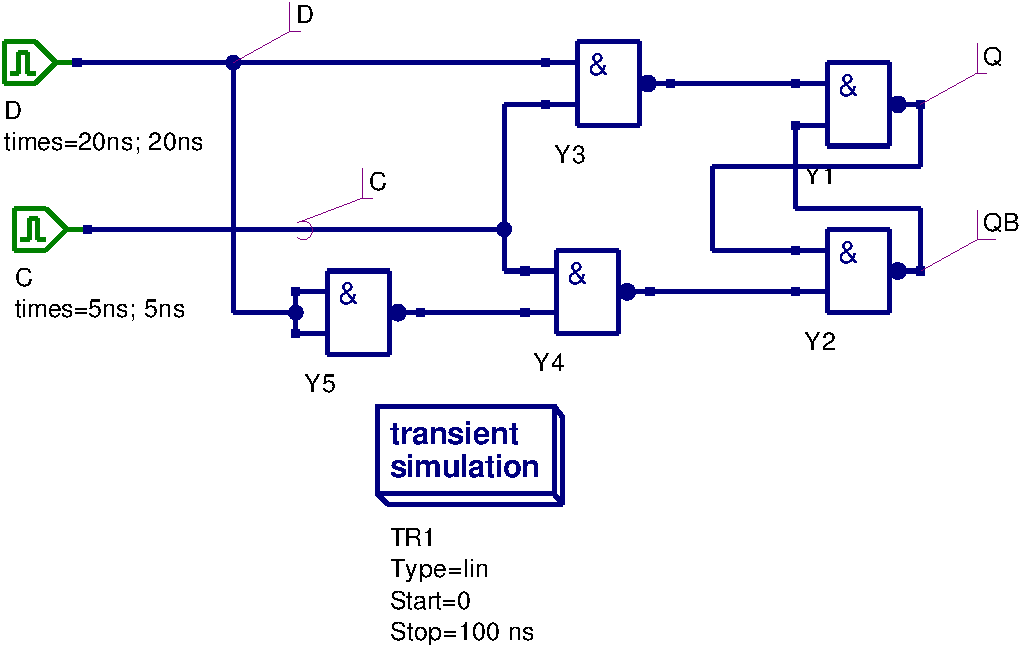
\includegraphics[width=0.7\linewidth]{fig1}
% fig1.ps: 72dpi, width=29.70cm, height=42.02cm, bb=0 0 842 1191
        \caption{Gated D latch with digital signal generators D and C}
  \label{fig:fig1}
\end{figure} 

\begin{figure}[ht]
  \centering
	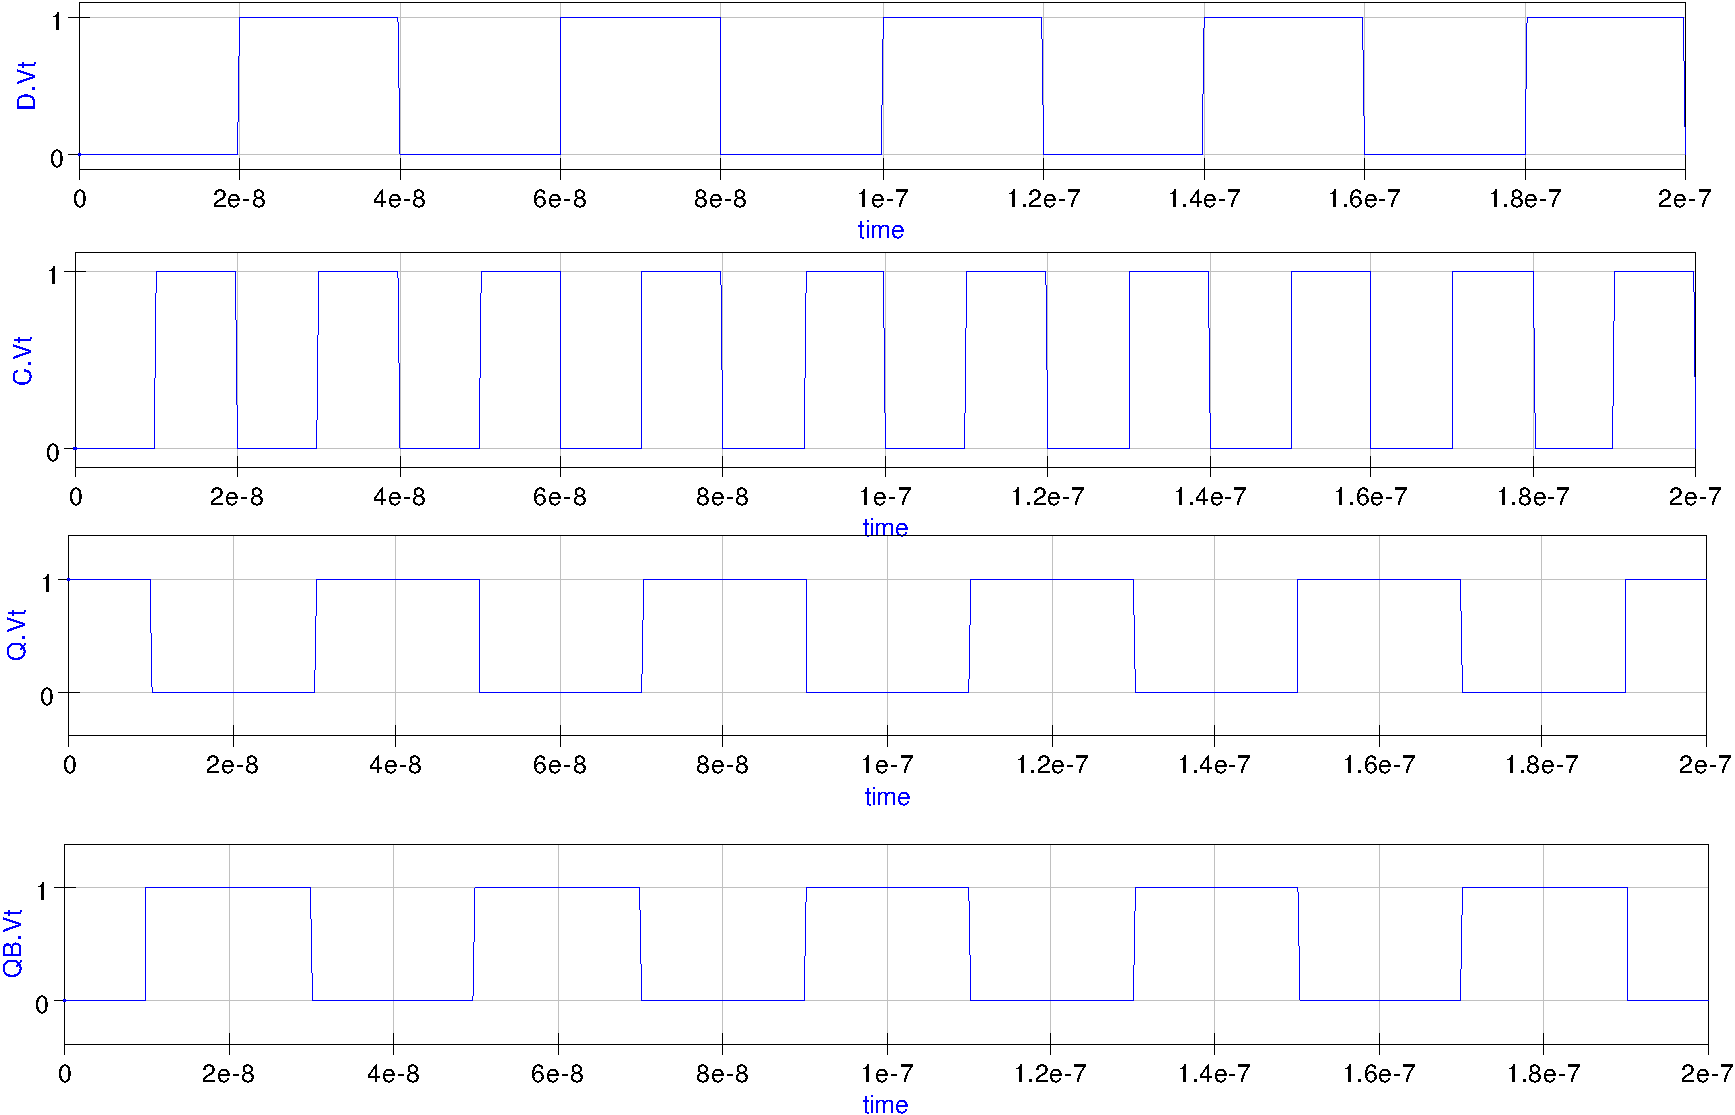
\includegraphics[width=1.0\linewidth]{fig3}
% fig2.pdf: 72dpi, width=13.48cm, height=4.69cm, bb=0 0 382 133
        \caption{Gated D latch simulation waveforms}
        \label{fig:fig3}
\end{figure} 

\begin{figure}[ht]
  \centering
  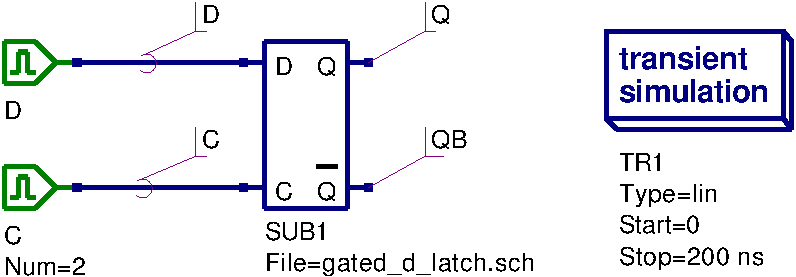
\includegraphics[width=0.8\linewidth]{fig2}
% fig3.pdf: 72dpi, width=29.56cm, height=18.94cm, bb=0 0 838 537
        \caption{Gated D latch test circuit}
        \label{fig:fig2}
\end{figure}

\tutsection{Edge-triggered D type flip-flop}

The schematic for a positive edge-triggered D flip-flop is shown in
Fig.~\ref{fig:fig4}\footnote{David A. Hodges and Horace G. Jackson,
Analysis and Design of Digital Integrated Circuits, 1998, Second
edition, McGraw-Hill Book Company.}. Asynchronous set (SET) and reset
(RESET) control inputs allow the flip-flop outputs Q and not Q (QB in
Fig.~\ref{fig:fig4}) to be set to known values at the start of a
simulation. The nand gates forming each of the cross coupled SR
latches have their delay times set at 0 ns. The edge-triggered D
device is a building block for both the JK and T types of flip-flop.
A typical set of transient simulation test results for the D flip-flop
model are illustrated in Fig.~\ref{fig:fig5}.  These where obtained
using the basic test configuration shown in Fig.~\ref{fig:fig6}.

\begin{figure}[ht]
  \centering
	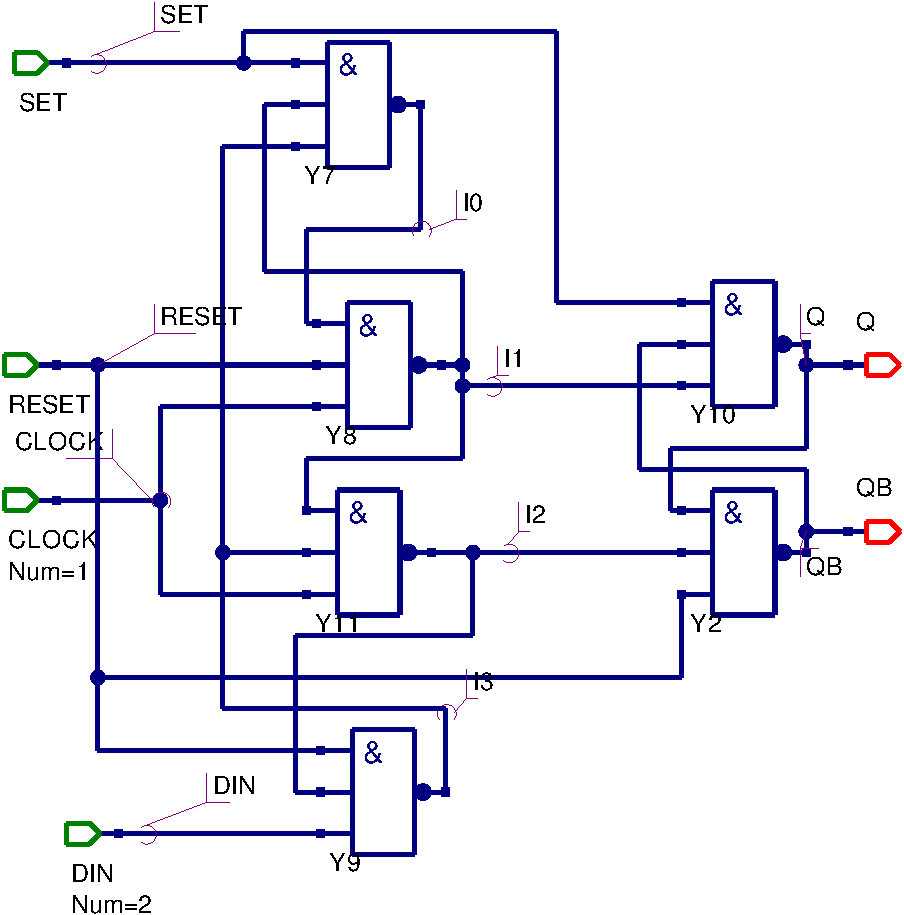
\includegraphics[width=0.8\linewidth]{fig4}
% fig4.pdf: 72dpi, width=15.31cm, height=15.49cm, bb=0 0 434 439
        \caption{Positive edge-triggered D flip-flop circuit}
        \label{fig:fig4}
\end{figure} 

\begin{figure}[ht]
  \centering
  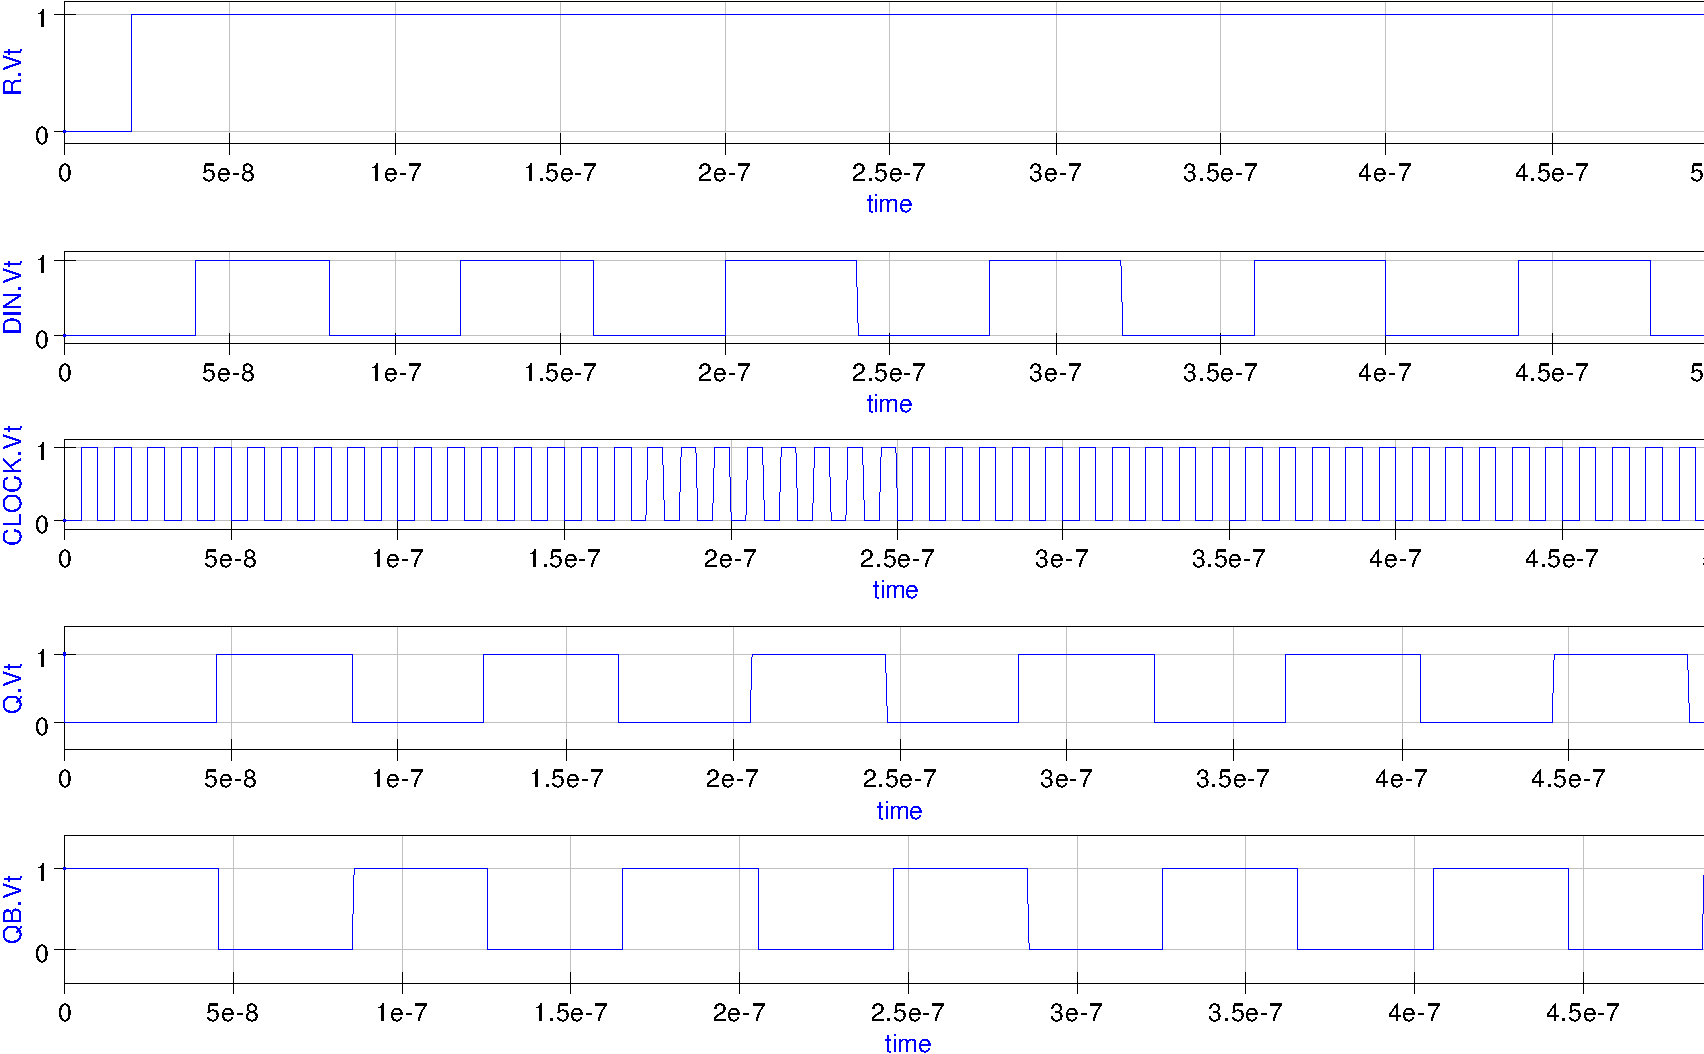
\includegraphics[width=1\linewidth]{fig5}
  \caption{Transient waveforms for the circuit shown in Fig.~\ref{fig:fig6}}
  \label{fig:fig5}
\end{figure}

\begin{figure}[ht]
  \centering
  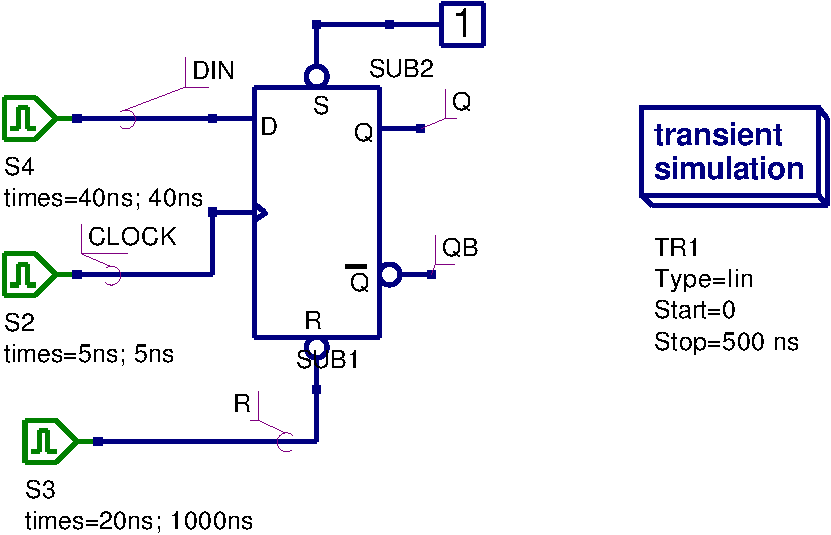
\includegraphics[width=0.7\linewidth]{fig6}
  \caption{D flip-flop test circuit}
  \label{fig:fig6}
\end{figure}

\FloatBarrier

\tutsection{The edge-triggered JK flip-flop}

A leading edge-triggered JK flip-flop can be constructed using a
positive edge-triggered D flip-flop and external
logic\footnote{M. Morris Mano and Charles R Kime, Logic and Computer
Design Fundamentals, 2004, Third edition, Pearson Education
International, Prentice Hall}. The external logic generates the
required JK flip-flop characteristic equation given by
\begin{center}
\begin{large}$Q^{+}=J.\overline{Q}+\overline{K}.Q$
\end{large}\end{center}
Were Q, $\overline{Q}$, J and $\overline{K}$ are the current state
values of the device signals and $Q^{+}$ is the next state value of Q
following the rising edge of the device clock pulse.  The schematic
diagram for the edge triggered flip flop is shown in
Fig.~\ref{fig:fig7} and a typical set of test waveforms in
Fig.~\ref{fig:fig8}. These were obtained using the test circuit shown
in Fig.~\ref{fig:fig9}.

\begin{figure}[ht]
  \centering
	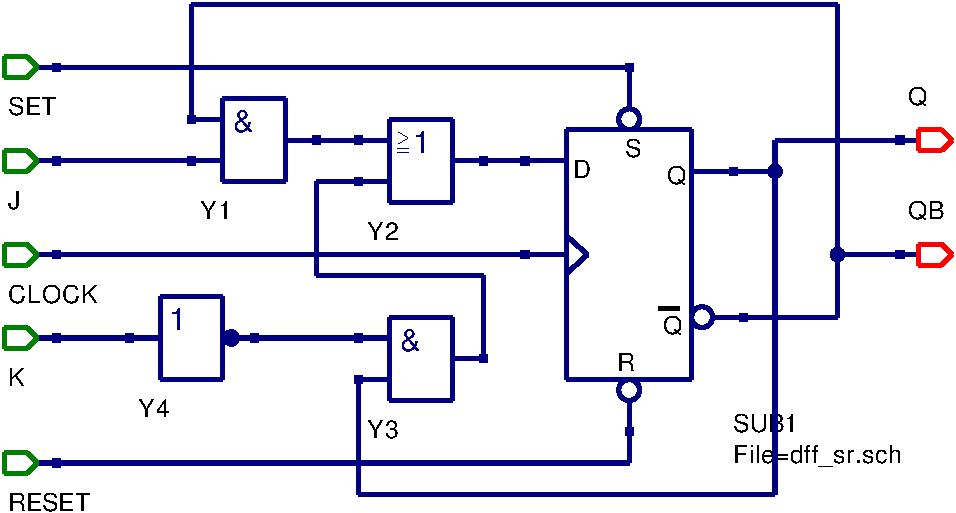
\includegraphics[width=0.8\linewidth]{fig7}
% fig4.pdf: 72dpi, width=15.31cm, height=15.49cm, bb=0 0 434 439
        \caption{Positive edge-triggered JK flip-flop circuit}
        \label{fig:fig7}
\end{figure} 

\begin{figure}[ht]
  \centering
  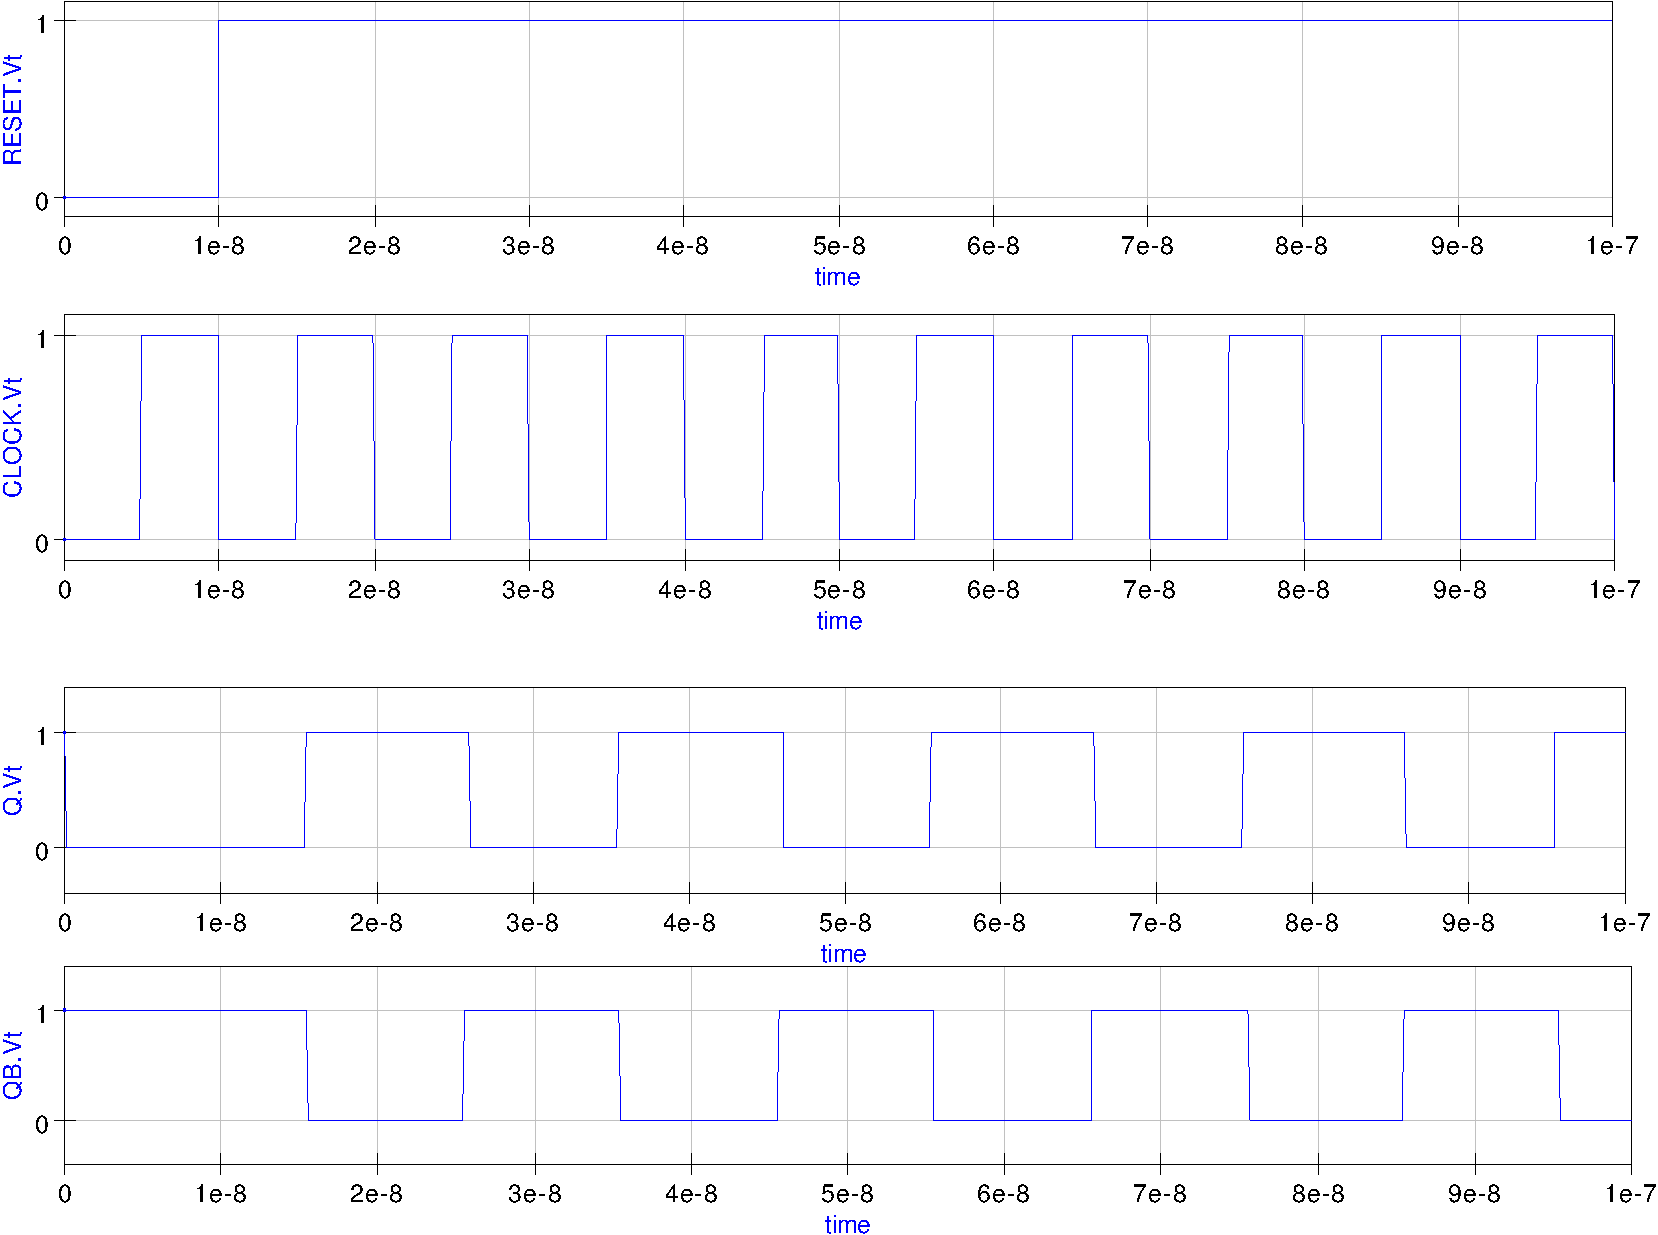
\includegraphics[width=0.9\linewidth]{fig8}
  \caption{Transient waveforms for the circuit shown in Fig.~\ref{fig:fig9}}
  \label{fig:fig8}
\end{figure}

\begin{figure}[ht]
  \centering
  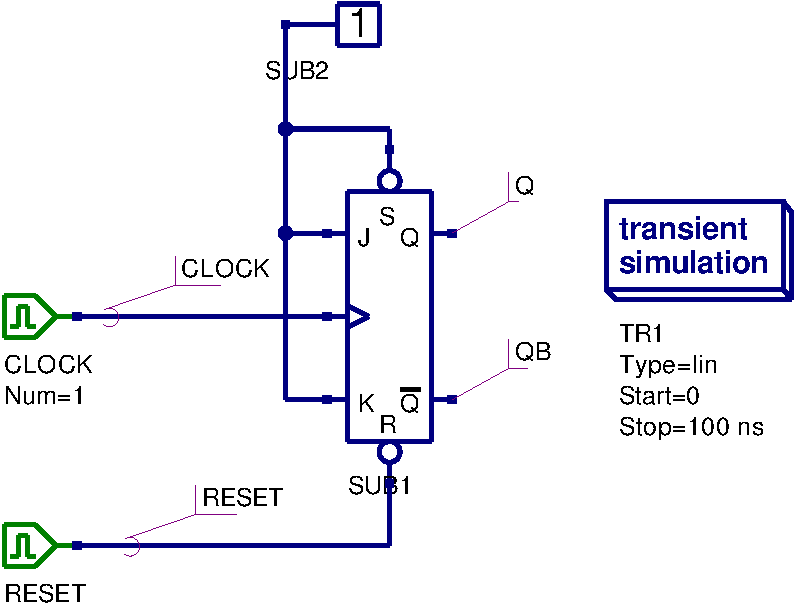
\includegraphics[width=0.7\linewidth]{fig9}
  \caption{JK flip-flop test circuit showing JK operating in toggle mode}
  \label{fig:fig9}
\end{figure}

\FloatBarrier

\tutsection{The edge-triggered T flip-flop}

The characteristic equation for a leading edge-triggered flip-flop
is\footnote{See footnote 2.}
\begin{center}
\begin{large}$Q^{+}=T \oplus Q$
\end{large}\end{center}
where the symbols have the same meaning as the JK flip-flop.  The
circuit diagram, test waveforms and test circuit for the
edge-triggered flip-flop are given in Figures~\ref{fig:fig10} to
\ref{fig:fig12}.

\begin{figure}[ht]
  \centering
	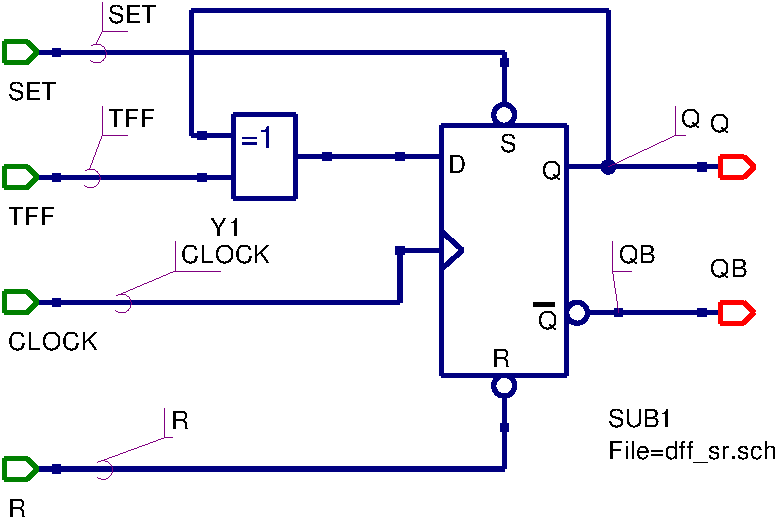
\includegraphics[width=0.7\linewidth]{fig10}
% fig4.pdf: 72dpi, width=15.31cm, height=15.49cm, bb=0 0 434 439
        \caption{Positive edge-triggered T flip-flop circuit}
        \label{fig:fig10}
\end{figure} 

\begin{figure}[ht]
  \centering
  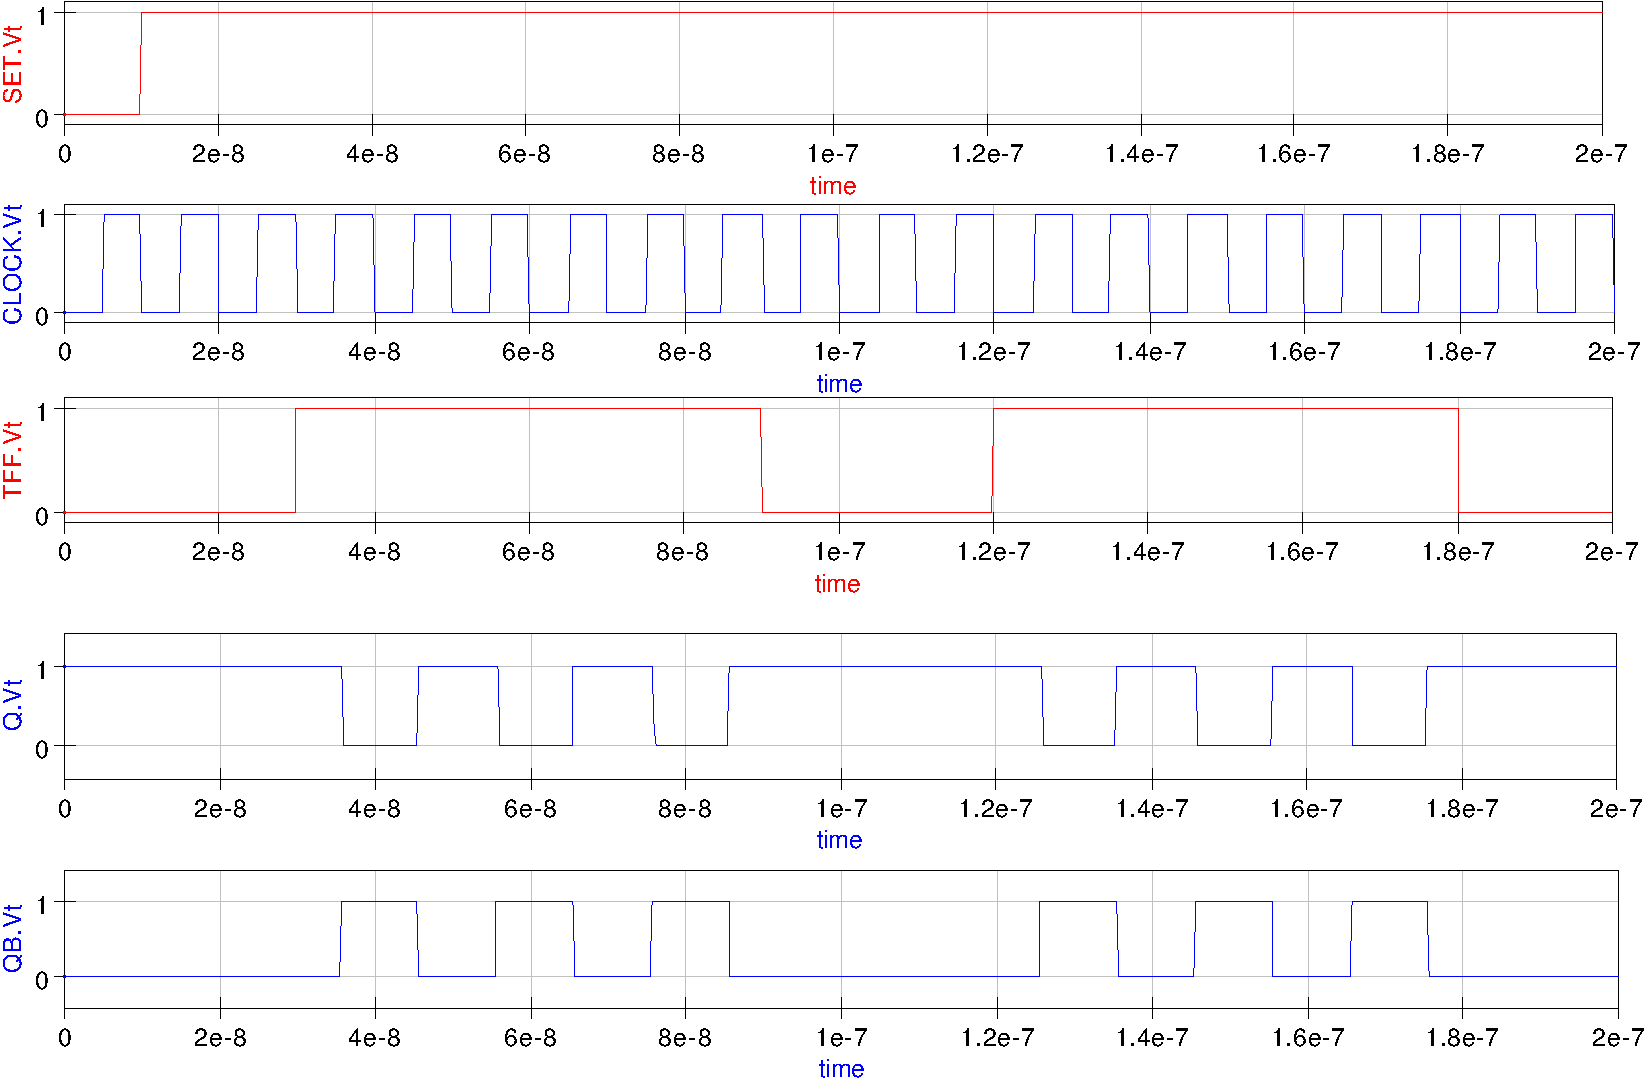
\includegraphics[width=1\linewidth]{fig11}
  \caption{Transient waveforms for the circuit shown in Fig.~\ref{fig:fig12}}
  \label{fig:fig11}
\end{figure}

\begin{figure}[ht]
  \centering
  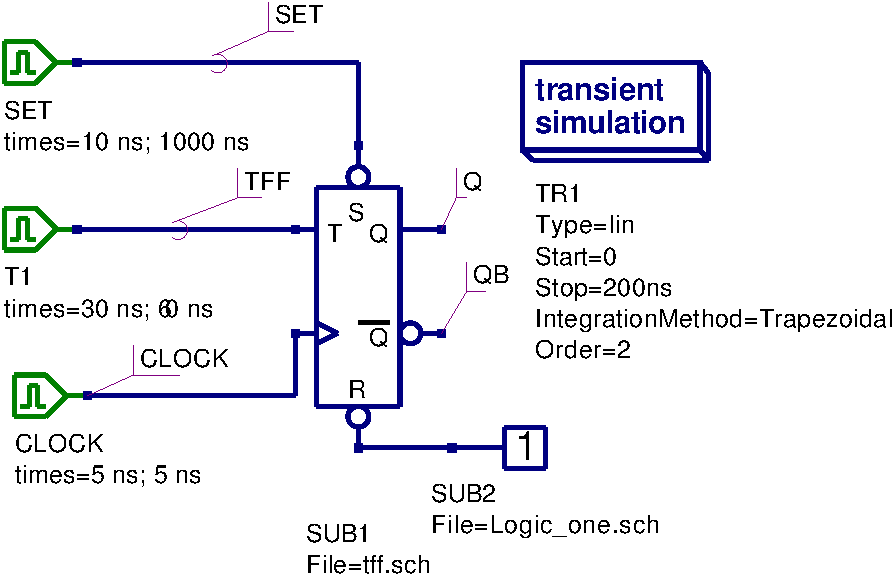
\includegraphics[width=0.7\linewidth]{fig12}
  \caption{T flip-flop test circuit}
  \label{fig:fig12}
\end{figure}

\tutsection{Two example digital circuits}
\begin{itemize}
\item
\textbf{A synchronous BCD up-counter}:
Figure~\ref{fig:fig13} shows a synchronous BCD up-counter constructed
from four edge-triggered JK flip flops connected as toggle
flip-flops. The input signal waveforms and the corresponding counter
outputs Q0, Q1, Q2 and Q3 are illustrated in Fig.~\ref{fig:fig14}.
These simulation results were obtained using the default trapezoidal
integration method with order 2.

\begin{figure}[ht]
  \centering
	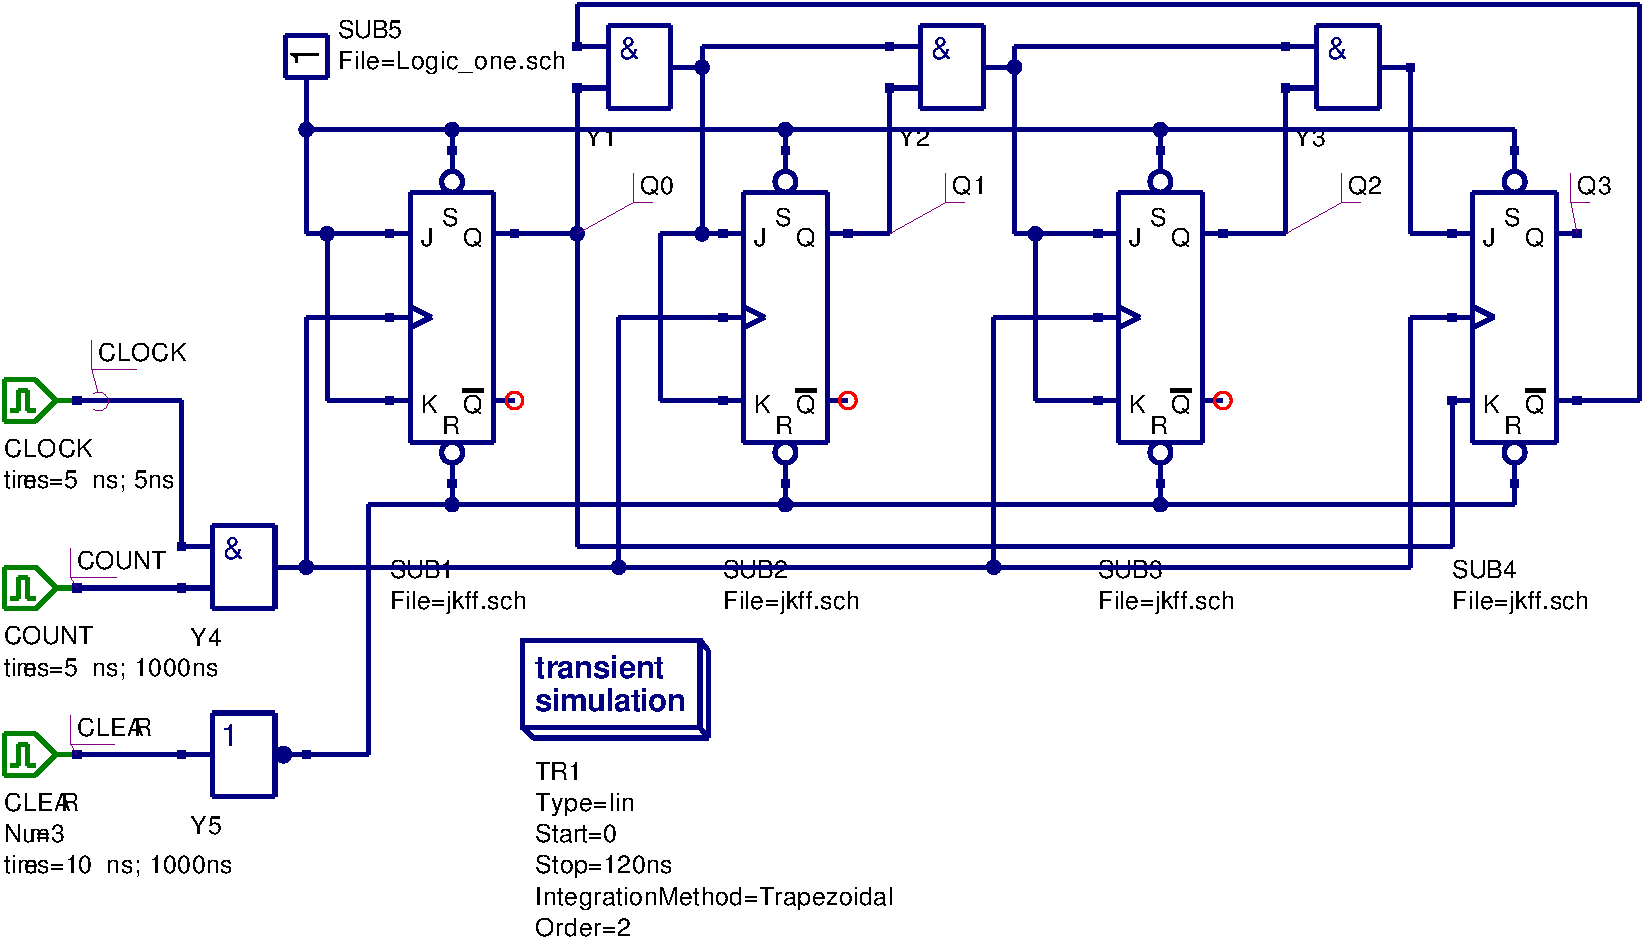
\includegraphics[width=1\linewidth]{fig13}
% fig4.pdf: 72dpi, width=15.31cm, height=15.49cm, bb=0 0 434 439
        \caption{Synchronous BCD up-counter circuit}
        \label{fig:fig13}
\end{figure} 

At the start of simulation signal CLEAR is set to logic 1 which in
turn causes the counter to be reset to 0000.  Similarly signal COUNT
has to be set to 1 for counting to take place. Notice that the counter
counts from 0 to 9 and then resets to 0.

\begin{figure}[ht]
  \centering
  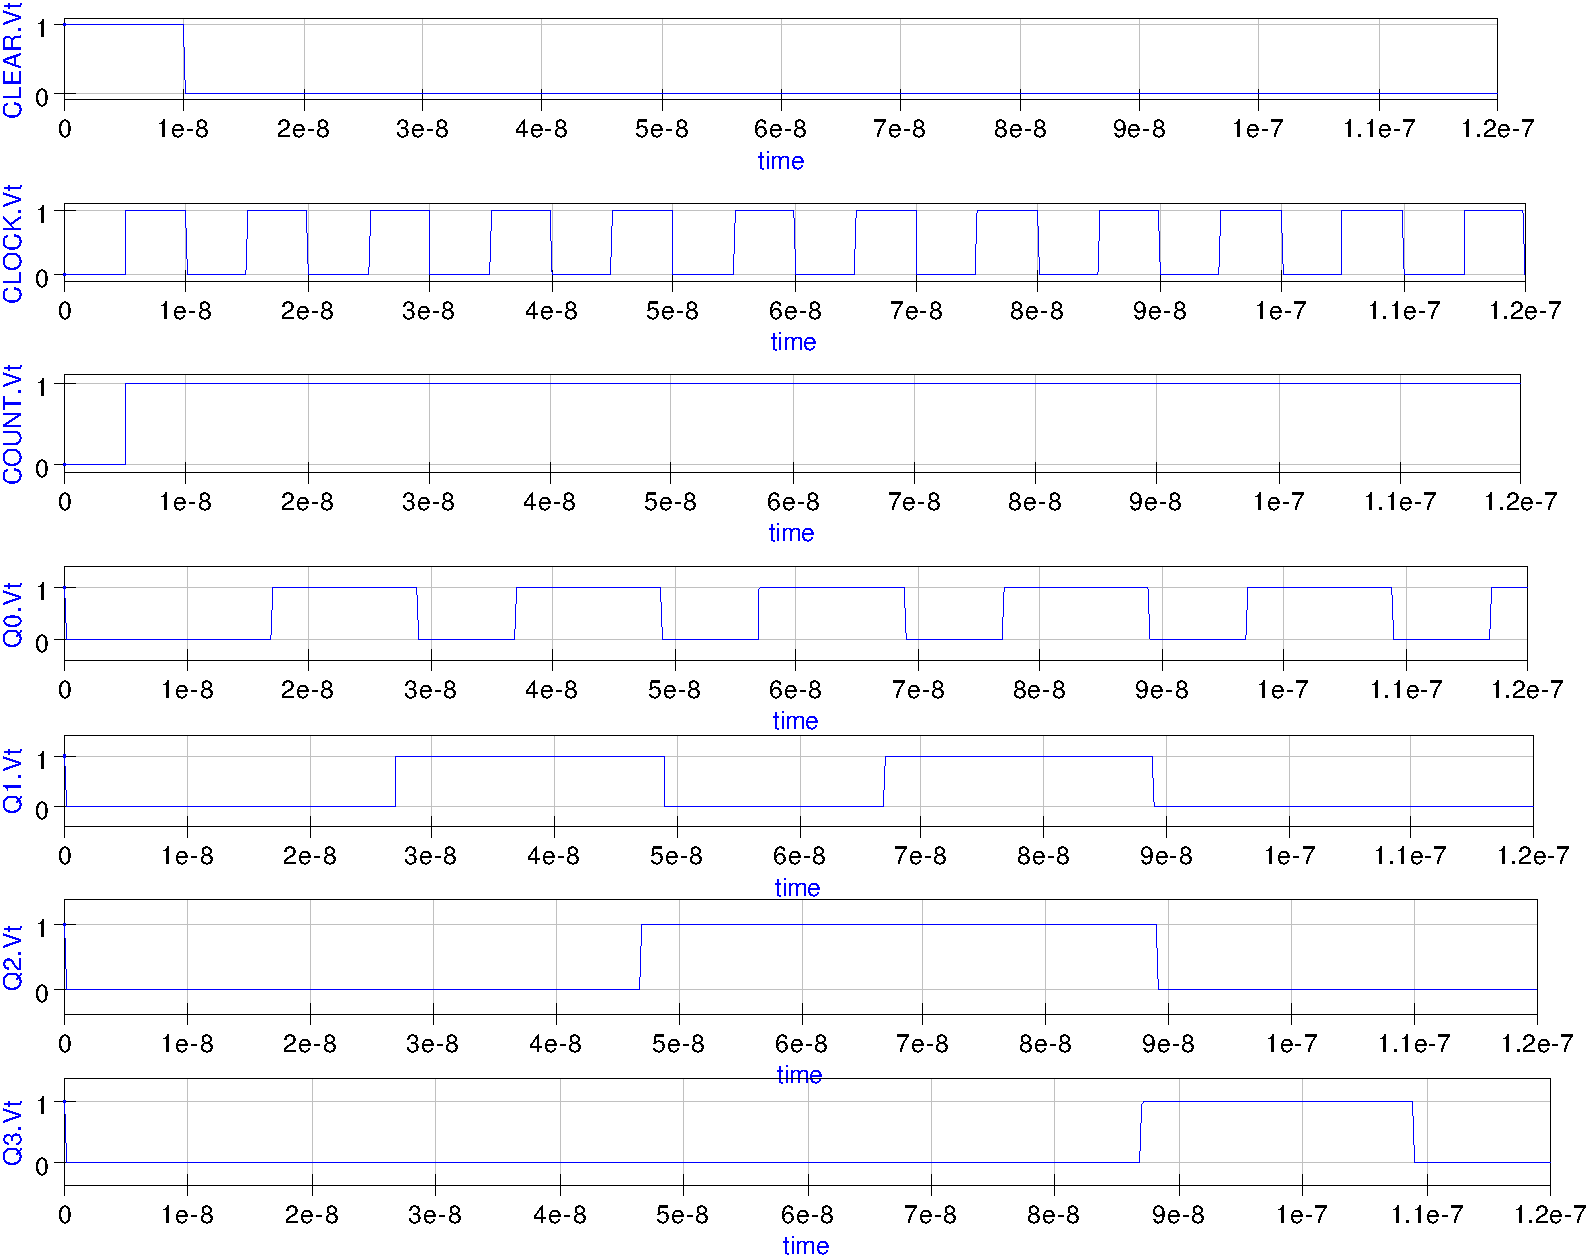
\includegraphics[width=1.0\linewidth]{fig14}
  \caption{Transient waveforms for the circuit shown in Fig.~\ref{fig:fig13}}
  \label{fig:fig14}
\end{figure}

\item
\textbf{A simple state machine}:
Figure~\ref{fig:fig15} shows a simple sequential state machine with
input X and outputs Y1 and Y2.  The outputs are synchronised to the
input clock.  The state equations for this example are

\begin{center}
\begin{large}
$J = \overline{X}$,  $K=1$,  $Y1=\overline{Q0}.\overline{X}$, $Y2=Q0$
\end{large}
\end{center}
\end{itemize}

\begin{figure}[ht]
  \centering
	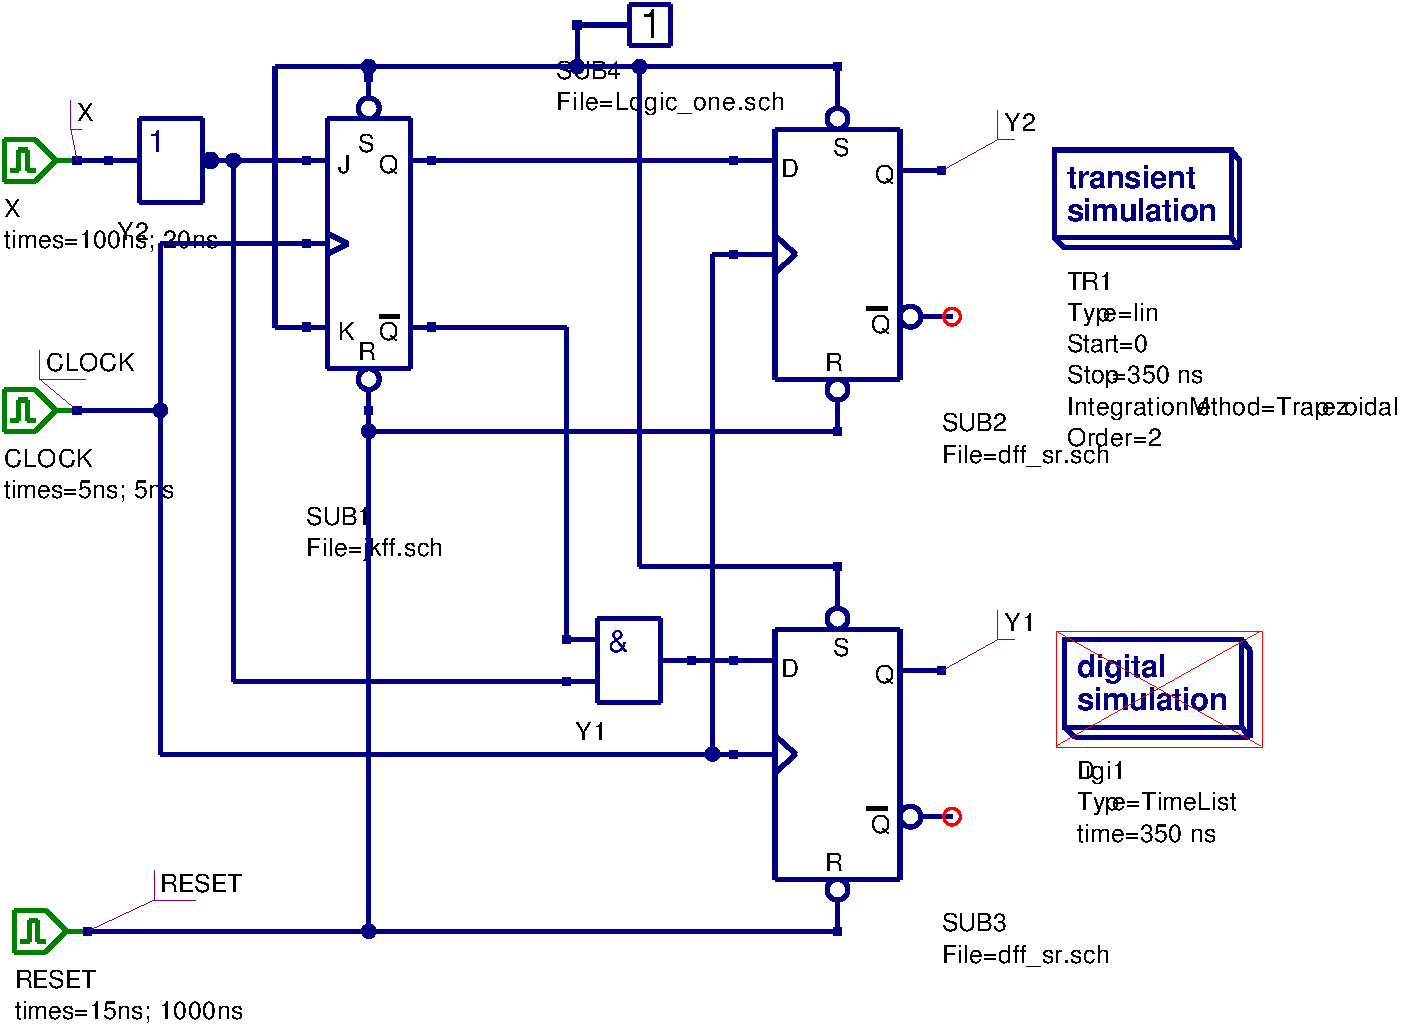
\includegraphics[width=1\linewidth]{fig15}
% fig4.pdf: 72dpi, width=15.31cm, height=15.49cm, bb=0 0 434 439
        \caption{A simple state machine}
        \label{fig:fig15}
\end{figure} 

\begin{figure}[ht]
  \centering
  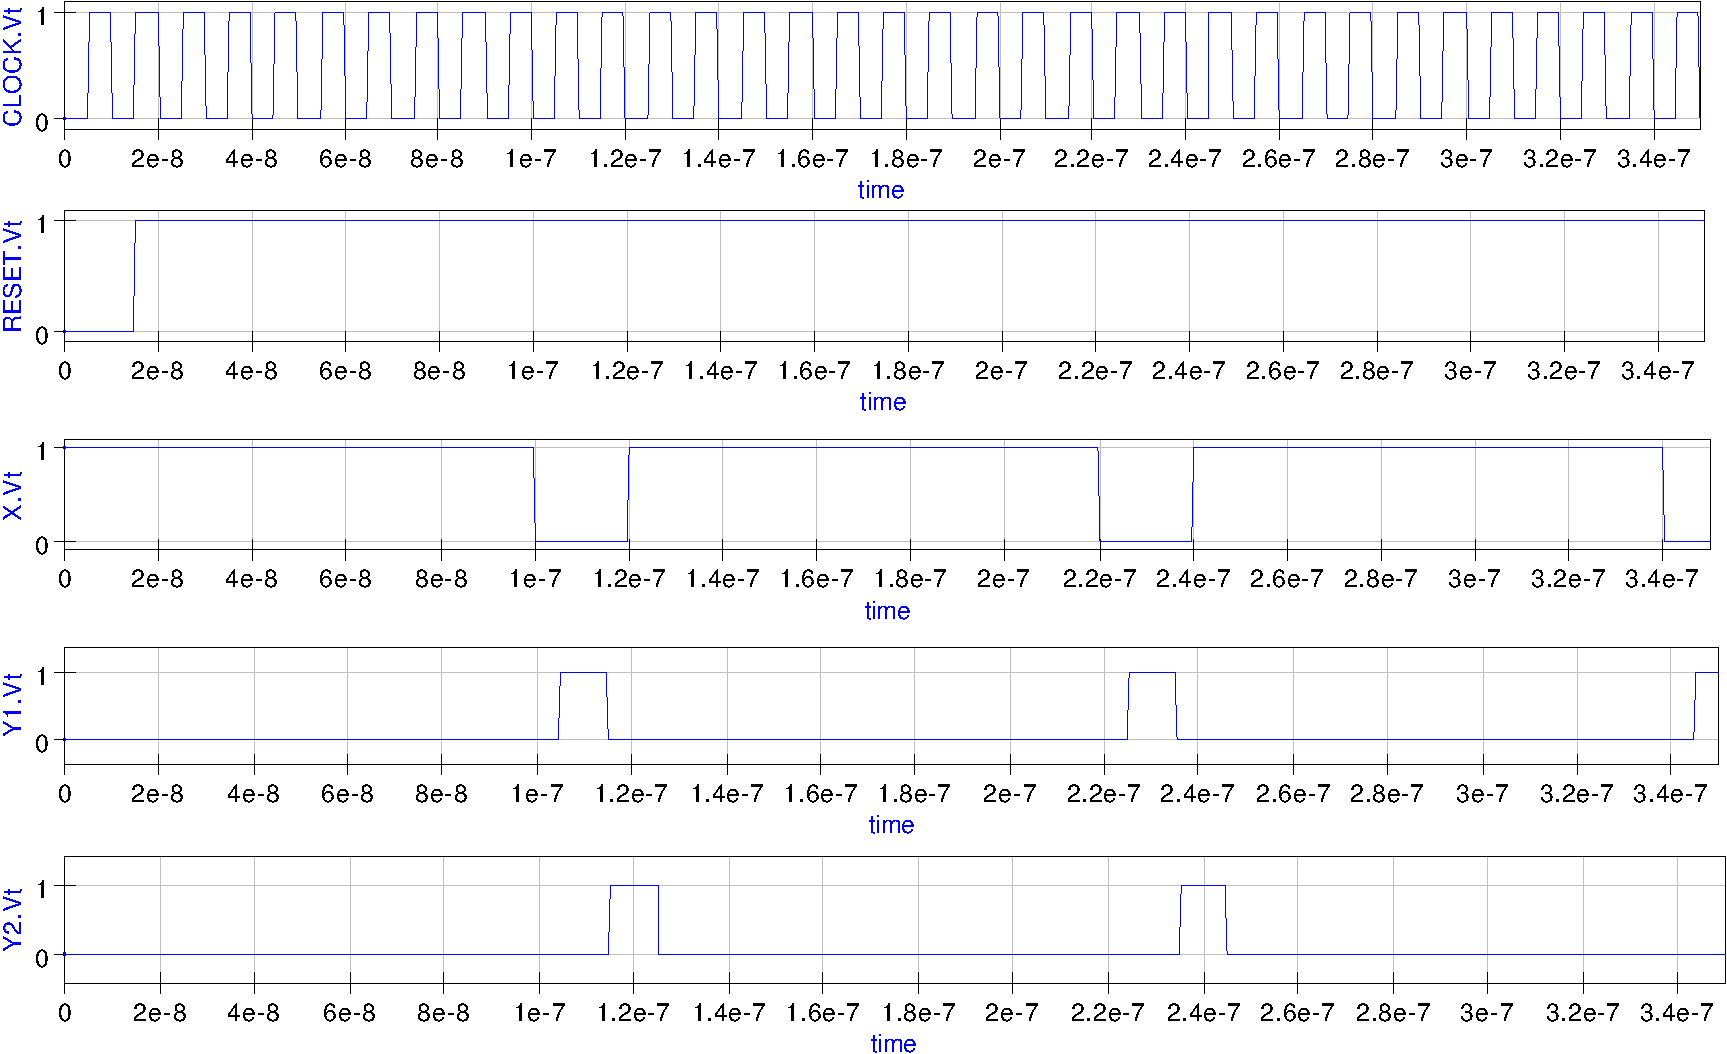
\includegraphics[width=1.0\linewidth]{fig16}
  \caption{Transient waveforms for the circuit shown in Fig.~\ref{fig:fig15}}
  \label{fig:fig16}
\end{figure}

\tutsection{VHDL code for the transient domain flip-flop models}
Although the primary purpose for developing the transient domain
flip-flop models is the simulation of mixed-mode circuits, it is worth
noting that because the models have been constructed from Qucs gate
primitives using a bottom-up design approach, Qucs can also use the
models for digital simulation.  Moreover, provided the circuit being
simulated does not contain any purely analogue components Qucs will
generate a VHDL model testbench that describes the function and test
sequence for the circuit being simulated.  Shown in
Fig.~\ref{fig:fig17} is a digital timelist waveform plot for the
synchronous BCD up-counter introduced in the previous section of these
notes.  Listing~\ref{lst:lst1} lists the VHDL code generated by Qucs for
the synchronous BCD up-counter example.


\begin{figure}[ht]
  \centering
	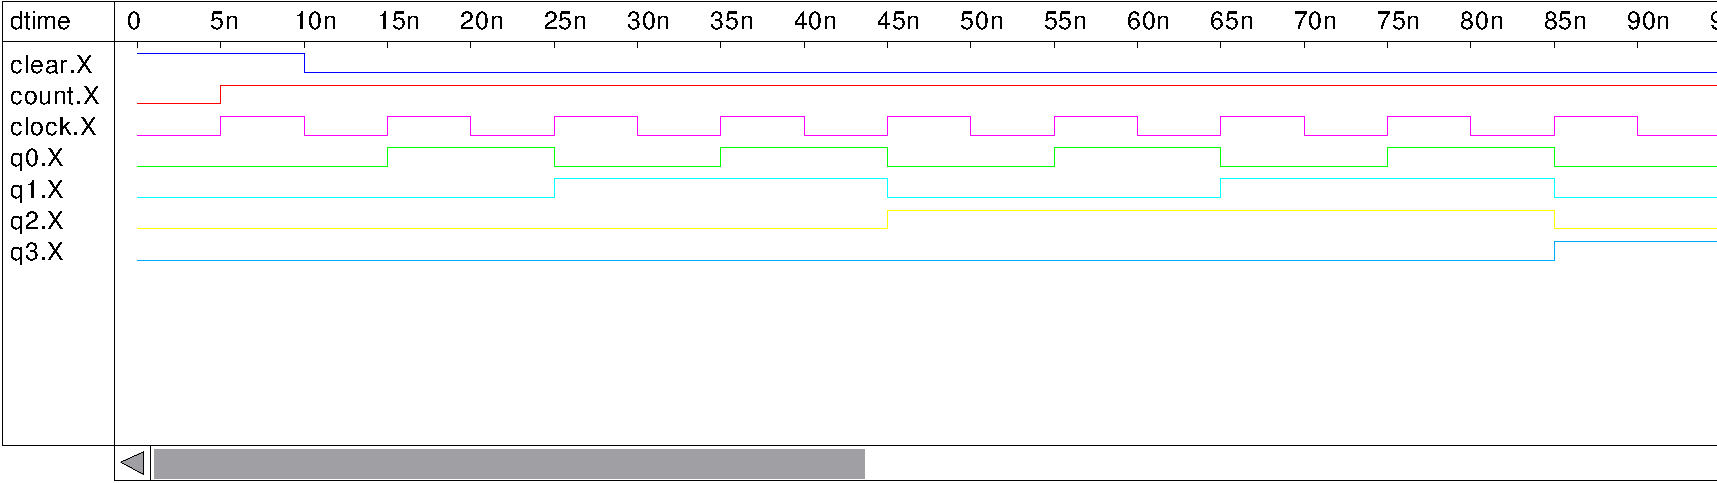
\includegraphics[width=1\linewidth]{fig17}
% fig4.pdf: 72dpi, width=15.31cm, height=15.49cm, bb=0 0 434 439
        \caption{Digital TimeList waveforms for the circuit shown in Fig.~\ref{fig:fig13}}
        \label{fig:fig17}
\end{figure} 

\begin{lstlisting}[language=VHDL,
    caption={VHDL testbench code for the circuit shown in Fig.~\ref{fig:fig13}},
    label={lst:lst1}]
-- Qucs 0.0.9  
-- /mnt/hda2/Digital_Subcircuits_prj/Sync_BCD_counter.sch

entity Sub_Logic_one is
  port (nnout_L1: out bit);
end entity;
use work.all;
architecture Arch_Sub_Logic_one of Sub_Logic_one is
  signal gnd,
         L1 : bit;
begin
  gnd <= '0';
  L1 <= not gnd;
  nnout_L1 <= L1 or '0';
end architecture;


entity Sub_dff_sr is
  port (CLOCK: in bit;
        DIN: in bit;
        nnout_Q: out bit;
        nnout_QB: out bit;
        RESET: in bit;
        SET: in bit);
end entity;
use work.all;
architecture Arch_Sub_dff_sr of Sub_dff_sr is
  signal I0,
         I2,
         I1,
         I3,
         QB,
         Q : bit;
begin
  nnout_QB <= QB or '0';
  nnout_Q <= Q or '0';
  I1 <= not (CLOCK and RESET and I0);
  I3 <= not (DIN and I2 and RESET);
  QB <= not (RESET and I2 and Q);
  Q <= not (I1 and QB and SET);
  I0 <= not (I3 and I1 and SET);
  I2 <= not (CLOCK and I3 and I1);
end architecture;


entity Sub_jkff is
  port (nnnet6: in bit;
        nnnet1: in bit;
        nnnet8: in bit;
        nnout_nnnet3: out bit;
        nnout_nnnet7: out bit;
        nnnet9: in bit;
        nnnet10: in bit);
end entity;
use work.all;
architecture Arch_Sub_jkff of Sub_jkff is
  signal nnnet0,
         nnnet2,
         nnnet4,
         nnnet5,
         nnnet7,
         nnnet3 : bit;
begin
  nnnet0 <= not nnnet1;
  nnnet2 <= nnnet3 and nnnet0;
  nnnet4 <= nnnet2 or nnnet5;
  nnnet5 <= nnnet6 and nnnet7;
  nnout_nnnet7 <= nnnet7 or '0';
  nnout_nnnet3 <= nnnet3 or '0';
  SUB1: entity Sub_dff_sr port map (nnnet8, nnnet4, nnnet3, 
                                    nnnet7, nnnet10, nnnet9);
end architecture;

entity TestBench is
end entity;
use work.all;

architecture Arch_TestBench of TestBench is
  signal CLEAR,
         COUNT,
         CLOCK,
         Q3,
         Q0,
         Q1,
         Q2,
         nnnet0,
         nnnet1,
         nnnet2,
         nnnet3,
         nnnet4,
         nnnet5,
         nnnet6,
         nnnet7,
         nnnet8,
         nnnet9 : bit;
begin
  SUB5: entity Sub_Logic_one port map (nnnet0);
  nnnet1 <= Q0 and nnnet2;
  nnnet3 <= Q1 and nnnet1;
  nnnet4 <= Q2 and nnnet3;
  SUB2: entity Sub_jkff port map (nnnet1, nnnet1, nnnet5, 
                                  Q1, nnnet6, nnnet0, nnnet7);
  
  
  SUB3: entity Sub_jkff port map (nnnet3, nnnet3, nnnet5, 
                                  Q2, nnnet8, nnnet0, nnnet7);
  SUB1: entity Sub_jkff port map (nnnet0, nnnet0, nnnet5, 
                                  Q0, nnnet9, nnnet0, nnnet7);
  nnnet5 <= COUNT and CLOCK;
  nnnet7 <= not CLEAR;

  CLEAR:process
  begin
    CLEAR <= '1';  wait for 10 ns;
    CLEAR <= '0';  wait for 1000 ns;
  end process;


  COUNT:process
  begin
    COUNT <= '0';  wait for 5 ns;
    COUNT <= '1';  wait for 1000 ns;
  end process;


  CLOCK:process
  begin
    CLOCK <= '0';  wait for 5 ns;
    CLOCK <= '1';  wait for 5 ns;
  end process;

  SUB4: entity Sub_jkff port map (nnnet4, Q0, nnnet5, 
                                  Q3, nnnet2, nnnet0, nnnet7);
end architecture;
\end{lstlisting}

\tutsection{Generating a library of mixed-mode digital components}

The Qucs project facilities offer users a simple and convenient
approach to developing libraries of components that are linked by a
common theme; in these notes this is digital component models for
transient simulation. To form a library create a new folder, at a
point on a disk file system that users have read/write access, giving
it a suitable name, for example
\begin{lstlisting}[language=clean] 
 flip_flop_models_tran_sim_prj. 
\end{lstlisting}  
Next move into the new library folder a copy of each of the schematic
capture files for the flip-flop models introduced in these notes.
These are:
\begin{lstlisting}[language=clean]
dff_sr.sch, jkff.sch, tff.sch, and gated_d_latch.sch.
\end{lstlisting} 

A copy of the schematic for setting nodes to logic one is also required 
\begin{lstlisting} [language=clean] 
( logic_one.sch ). 
\end{lstlisting}

These models are then freely available for use in any projects which
users are working on.  They can be copied into such projects using the
"Add files to Project..." menu button found under the Qucs Project
drop-down menu. Similarly any new models developed as part of a
project can be added to the library and used again in the future.

\tutsection{Digital component propagation time delays and transient simulation numerical stability}

Transient simulation is in general much slower than digital simulation
using VHDL generated machine code. The large signal transient
simulation models of flip-flops and other sequential digital devices
are intended for use in mixed-mode circuit simulation rather than
being used for pure digital circuit simulation.  An interesting, and
indeed very important question, relates to the efficiency, and
accuracy, of the numerical analysis algorithms employed in the
integration routines that are central to transient circuit simulation.
Qucs allows users to select the algorithm they wish to employ for
transient simulation.  The available algorithms are Trapezoidal,
Euler, Gear and Adams Moulton; in each case the algorithm order can be
set from 1 to 6. The second order Trapezoidal integration algorithm is
used by Qucs as the default for transient simulation. To test which of
these algorithms offers the most time efficient solution to the
transient simulation of digital circuits, that include flip-flops, the
BCD counter shown in Fig.~\ref{fig:fig13} was used as a test case and
repeatedly simulated using different integration routines and
algorithm orders. The test results are shown in Table~\ref{tab:tab2}.
Very little difference was found between circuits where the cross
coupled gates both had zero propagation delays and the case where one
gate had 0.5ns delay and the other zero delay.

\begin{table}
\begin{center}
% use packages: array
\begin{tabular}{lllll}
Order & Trapezoidal & Euler & Gear & Adams Moulton \\ 
1 & 1 & 1.62 & 1.65 & 1.62 \\ 
2 & 1 & 1.62 & 0.44 & 1 \\ 
4 & 1 & 1.62 & 1.28 & 0.39 \\ 
6 & 1 & 1.62 & 0.28 & 0.18 
\end{tabular}
\end{center}
\caption{Relative simulation times for the circuit shown in Fig.~\ref{fig:fig13}}
\label{tab:tab2}
\end{table}

\addvspace{12pt}

One obvious fact emerges from the data given in Table~\ref{tab:tab2};
namely that the Adams Moulton higher order integration routines appear
to be faster than the default trapezoidal algorithm.  This is
corroborated by the average time step and number of rejection data
points output by Qucs at the end of a simulation. Table~\ref{tab:tab3}
lists this data for the Adams Moulton algorithm tabulated in
Table~\ref{tab:tab2}.
\begin{table}
\begin{center}
% use packages: array
\begin{tabular}{lll}
Order & Number or rejections & Average time step \\ 
1 & 1470 & 5.17737e-12 \\ 
2 & 1750 & 9.4585e-12 \\ 
4 & 1454 & 2.866e-11 \\ 
6 & 61 & 5.76646e-11
\end{tabular}
\end{center}
\caption{Number of rejections and average time step data for the Adams Moulton algorithm}
\label{tab:tab3}
\end{table}

\addvspace{12pt}

Table~\ref{tab:tab3} points to the increase in average time step and
the dramatic reduction in the number of simulation solution rejections
as the probable reason for the reduction in transient simulation time
when using the higher order Adams Moulton integration routines.
However, other factors may influence the choice of integration
routine.  Often speed is not the only criteria that is of importance
when simulating large complex circuits.  Consider the following case
(the circuit shown in Fig.~\ref{fig:fig13} with order 6 Adams Moulton
transient analysis integration); setting one of the gate delays to
1ns, and the other to 0ns, in each of the RS latches in the
edge-triggered D flip-flop yields the signal waveforms illustrated in
Fig.~\ref{fig:fig18}. Clearly here the solution is incorrect pointing
to probable numerical instability caused by the choice of integration
routine.

\begin{figure}[ht]
  \centering
	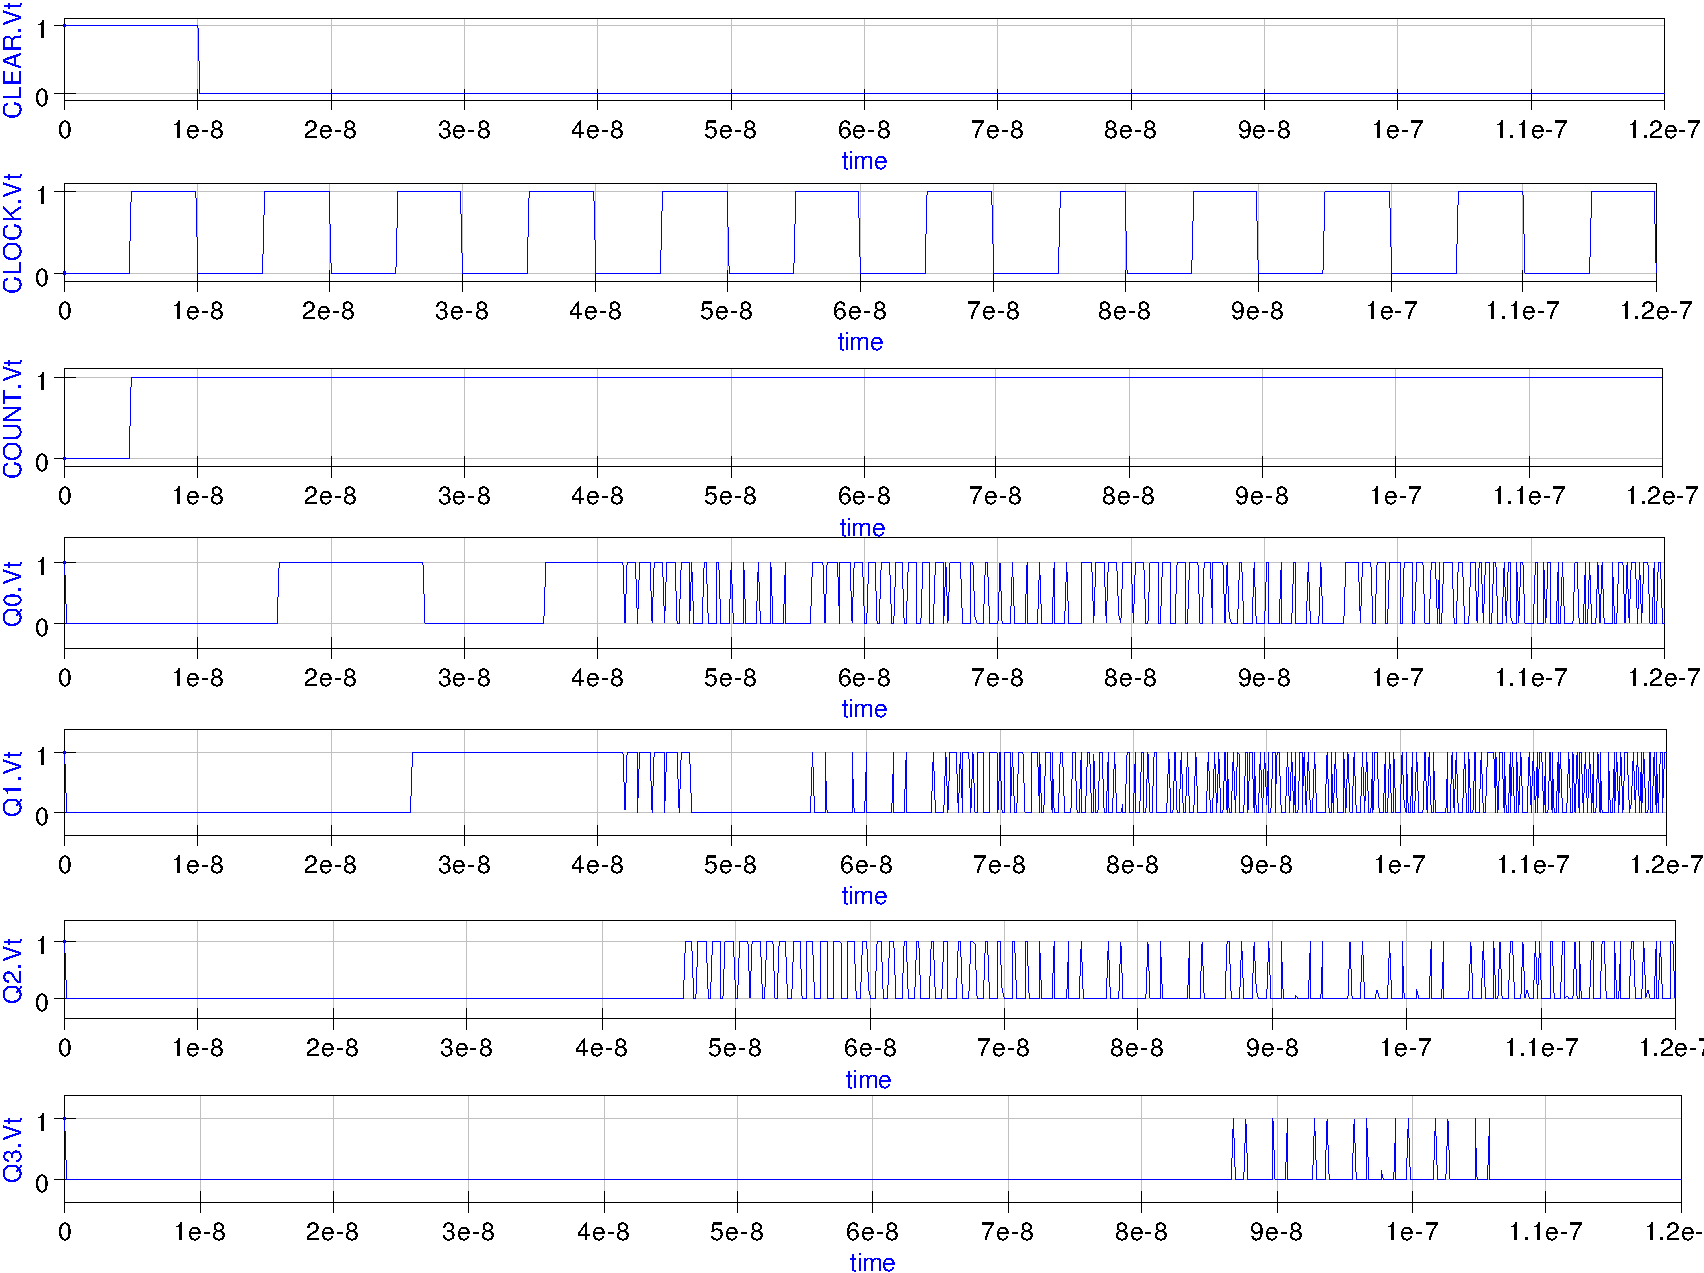
\includegraphics[width=0.75\linewidth]{fig18}
% fig18.pdf: 72dpi, width=28.86cm, height=21.55cm, bb=0 0 818 611
        \caption{Digital TimeList waveforms for the circuit shown in Fig.~\ref{fig:fig13}}
        \label{fig:fig18}
\end{figure} 

\tutsection{Mixed-mode example simulations}

Mixed-mode simulation involves the simulation of circuits that contain
electronic devices and circuits from different physical domains; the
most obvious being circuits with a mixture of analogue and digital
components.  Qucs has developed to a point where it can handle this
type of circuit given device models that can span across the different
physical domains. In the future such circuits are likely to
incorporate components from other domains, including for example,
digital signal processing components (DSP) and possibly nano
mechanical devices.  Multi-domain simulation adds additional
complexity to the simulation process not normally found in single
domain simulation.  Each domain usually represents signal data in a
specific way attributed to a given domain; voltage and current for
analogue quantities, boolean '1' and '0' for digital signals and
floating point numbers for DSP.  Hence, signals passing from one
domain to another have to be converted from one format to
another. These conversion elements are often called node-bridges and
form an essential part of the mixed-mode simulation process.  The
three examples that are introduced in this section of these notes have
been chosen to illustrate a number of the basic ideas concerned with
mixed-mode simulation of circuits containing analogue and digital
components, and to show how Qucs deals with this type of simulation.
In the last section the importance of correct selection of integration
routine when simulating circuits in the time domain was stressed.
Mixed-mode circuits often include a wide diversity of components that
exhibit widely differing time constants.  This makes the problem of
numerical stability versus simulation run time even more critical.
With the explicit numerical integration routines, like the trapezoidal
routine, numerical instability results if the simulation time step
becomes much larger than the smallest time constant in a circuit.
Hence, to achieve successful completion of a simulation the
integration time step must be reduced which in turn makes the overall
simulation time increase significantly.  The implicit Gear
algorithm\footnote{The Gear integration algorithm is a powerful method
for solving stiff systems of differential equations, see Donald
A. Calahan, Computer Aided Network Design, Revised edition, 1972,
McGraw-Hill.} does not suffer from this problem and is the natural
choice for circuits with components that have widely differing time
constants.

\begin{itemize}
\item Example 1: Analogue waveform driven digital devices with output node-bridge.

The circuit in Fig.~\ref{fig:fig19} shows an analogue voltage source
driving a digital inverter with a node-bridge element processing the
inverter output signal.  The input signal is a sinusoidal voltage of
amplitude 1V peak.  The inverter output signal, V1 in
Fig.~\ref{fig:fig19}, has an nonsymmetrical mark to space ratio
because the threshold point for the inverter is set at 0.5V; the
halfway point for the two logic levels.  The node-bridge element is
basically a voltage controlled voltage source where the device gain
and time delay can be programmed.  In this first example the gain has
been set to 5 and the time delay to 0.5ns.  Figure ~\ref{fig:fig20}
illustrates the simulation TimeList waveforms for this example
mixed-mode circuit. The node-bridge shown in Fig.~\ref{fig:fig19} is a
very basic device. Moreover, by adding additional features, parameters
like fall and rise time can set to specific values. The next example
demonstrates the use of an active node-bridge.

\begin{figure}[ht]
  \centering
	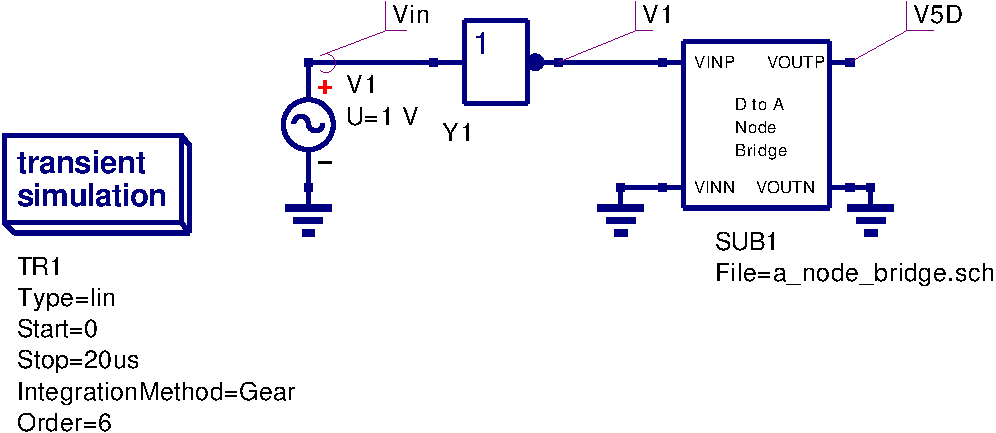
\includegraphics[width=0.9\linewidth]{fig19}
% fig18.pdf: 72dpi, width=28.86cm, height=21.55cm, bb=0 0 818 611
        \caption{Analogue waveform driven digital device with output node-bridge}
        \label{fig:fig19}
\end{figure} 

\begin{figure}[ht]
  \centering
	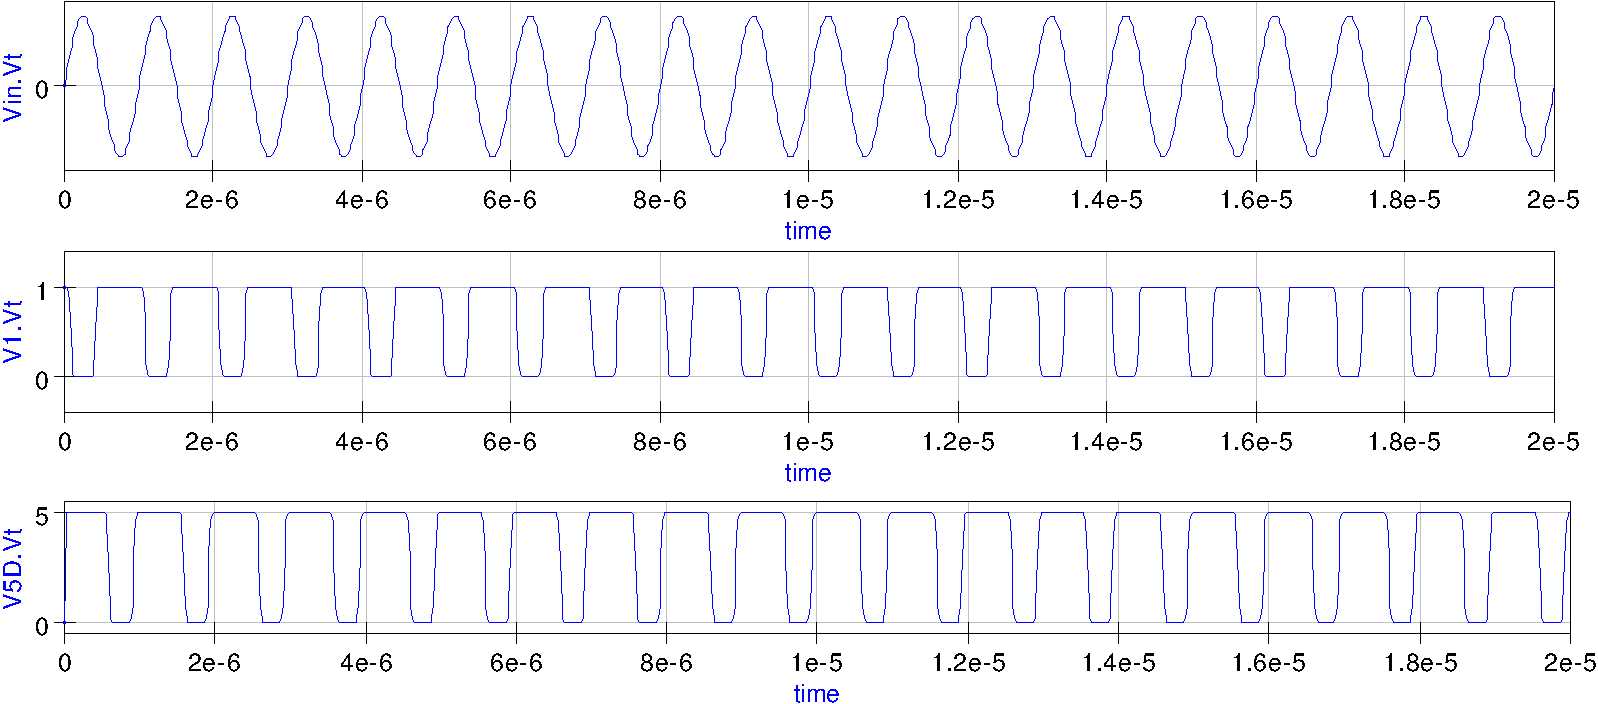
\includegraphics[width=1.0\linewidth]{fig20}
% fig18.pdf: 72dpi, width=28.86cm, height=21.55cm, bb=0 0 818 611
        \caption{Digital TimeList waveforms for the circuit shown in Fig.~\ref{fig:fig19}}
        \label{fig:fig20}
\end{figure} 
\FloatBarrier
\item Example 2: Pulse driven digital inverter with an active node bridge.

Illustrated in Fig.~\ref{fig:fig21} is a similar circuit to the
previous example.  In Fig.~\ref{fig:fig21} a pulse generator drives a
digital inverter. The inverter output signal is processed by an active
node-bridge derived from a basic BJT switching amplifier.  The output
waveforms for this circuit are shown in Fig.~\ref{fig:fig22}.  Notice
that the pulse rise and fall times are determined by the node-bridge
amplifier and that the resulting analogue signal amplitude is set to
5V.

\begin{figure}[ht]
  \centering
	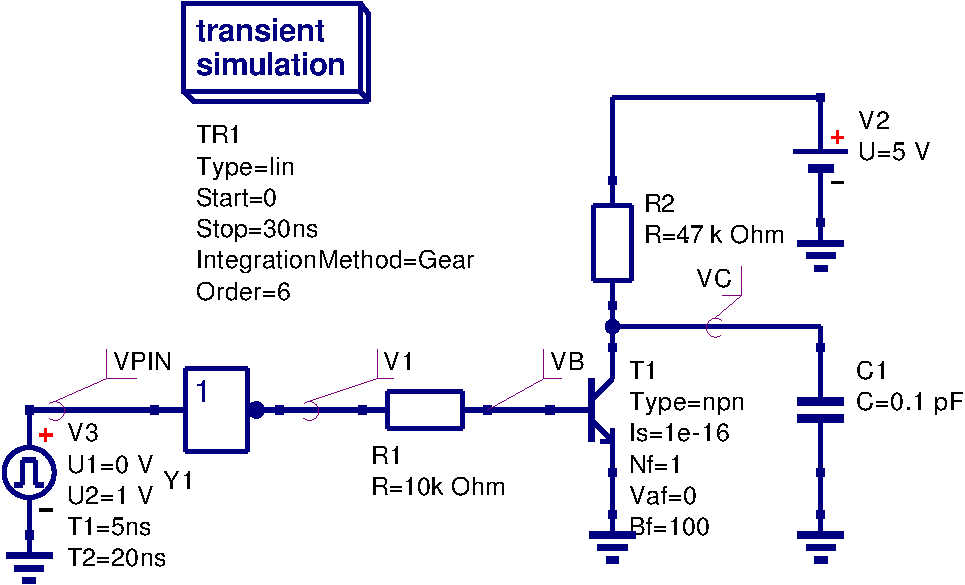
\includegraphics[width=0.9\linewidth]{fig21}
% fig18.pdf: 72dpi, width=28.86cm, height=21.55cm, bb=0 0 818 611
        \caption{Pulse driven digital inverter with active node-bridge}
        \label{fig:fig21}
\end{figure} 

\begin{figure}[ht]
  \centering
	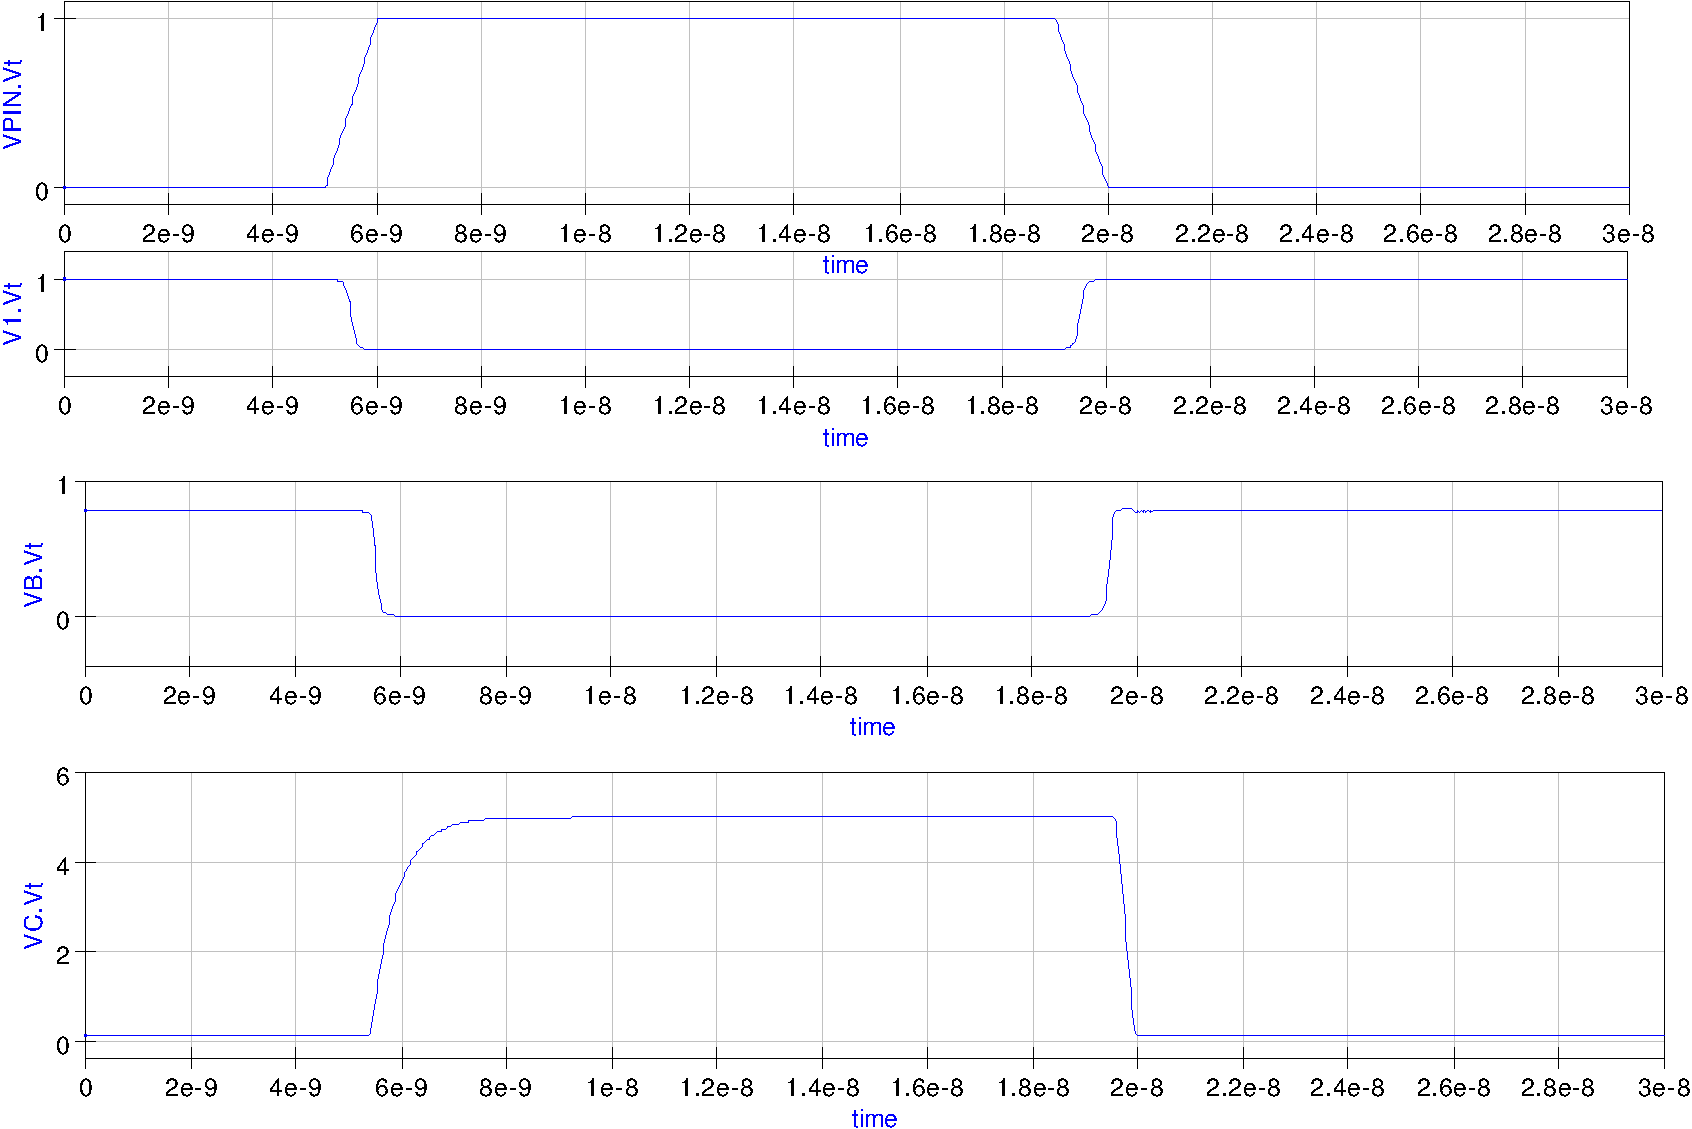
\includegraphics[width=1.0\linewidth]{fig22}
% fig18.pdf: 72dpi, width=28.86cm, height=21.55cm, bb=0 0 818 611
        \caption{Digital TimeList waveforms for the circuit shown in Fig.~\ref{fig:fig21}}
        \label{fig:fig22}
\end{figure} 
\FloatBarrier

\item Example 3: A more complex mixed-mode simulation example.

The circuit shown in Fig.~\ref{fig:fig23} brings together a number of
the ideas outlined in these tutorial notes.  A 4-bit digital signal is
generated from a simple asynchronous binary counter operated from a
digital clock signal.  The counter output is transformed to the
analogue domain using a simple node-bridge, of the type introduced in
mixed-mode example 1.  A 4-bit binary weighted DAC converts the
transformed node-bridge signals into the final analogue output signal.
The DAC operational amplifier is modelled as a gain block with a
single pole frequency response and DC voltage output limiting.  The
output waveforms for this example are shown in Fig.~\ref{fig:fig24}
and the details of the operational amplifier model in
Fig.~\ref{fig:fig25}.
\begin{figure}[ht]
  \centering
	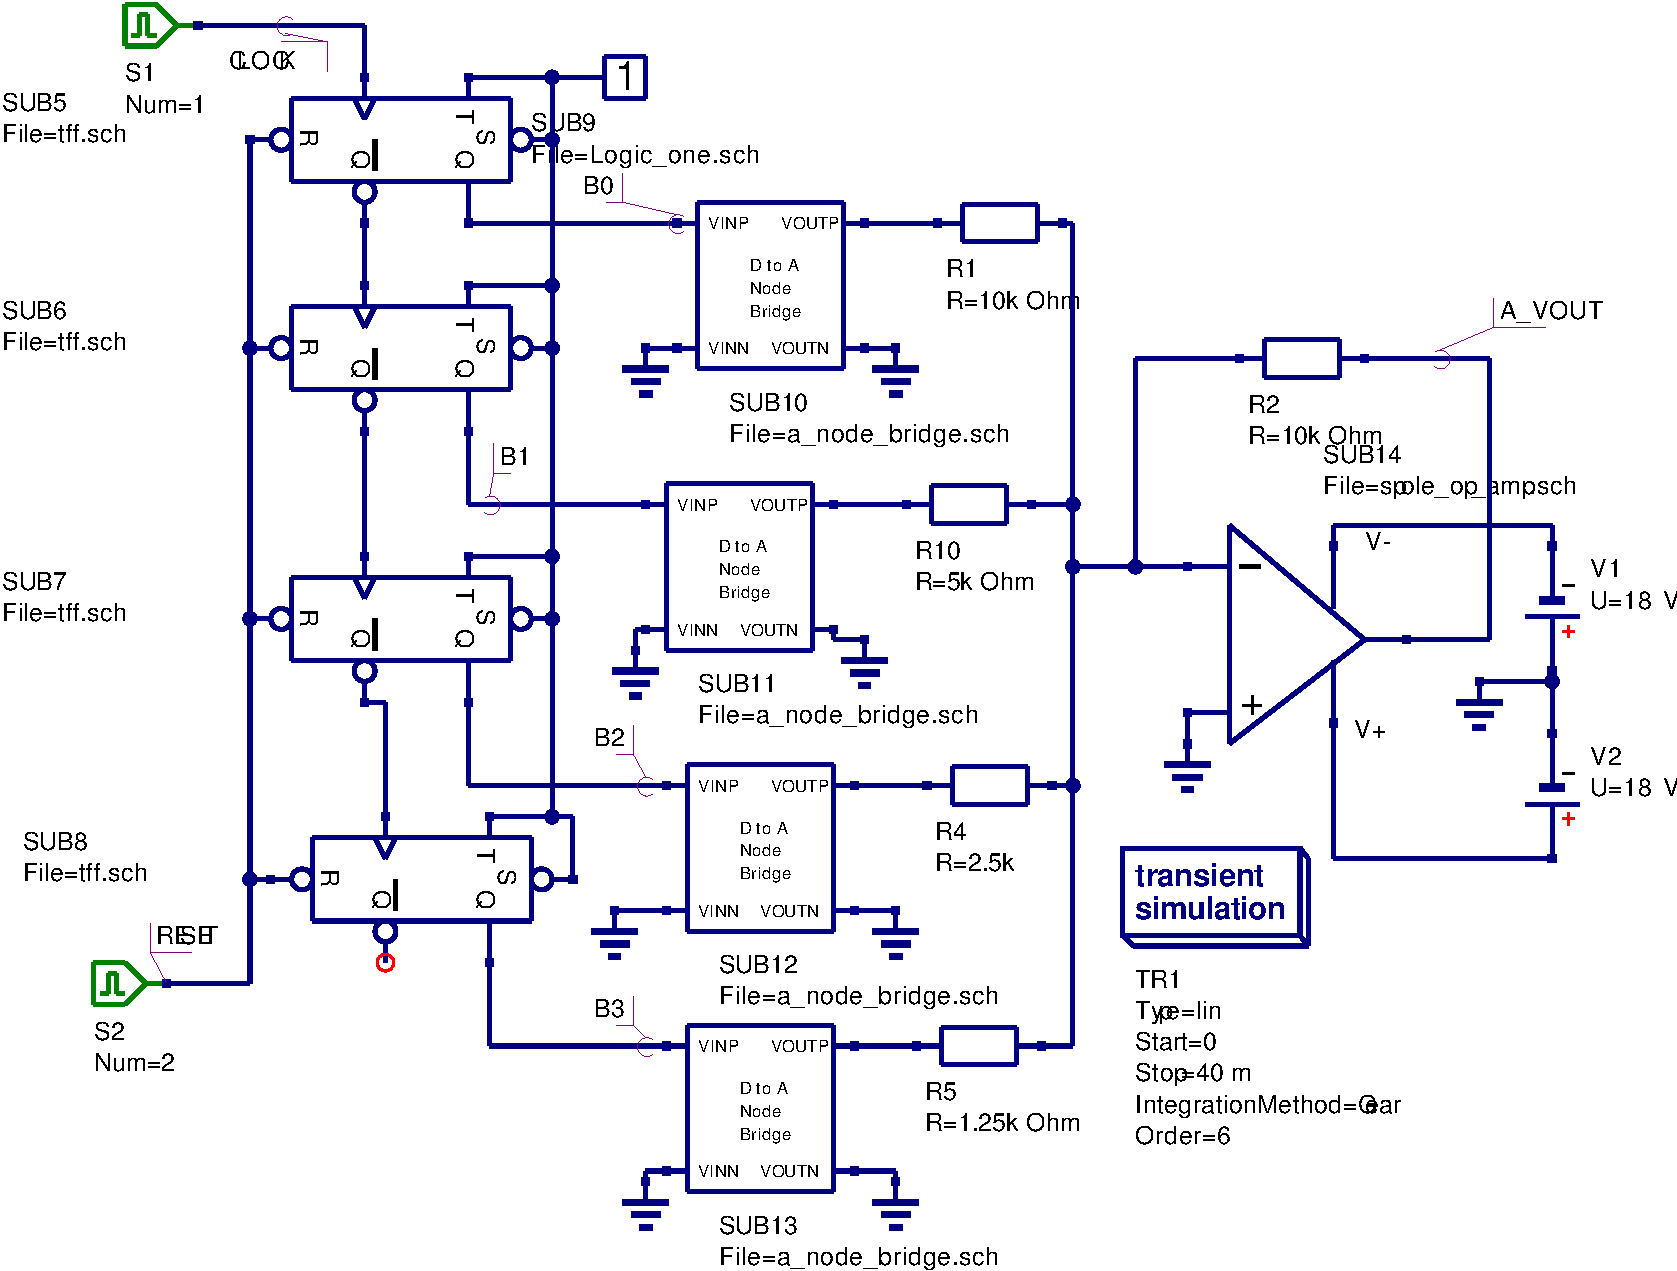
\includegraphics[width=1.0\linewidth]{fig23}
% fig18.pdf: 72dpi, width=28.86cm, height=21.55cm, bb=0 0 818 611
        \caption{A more complex analogue-digital mixed-mode simulation example}
        \label{fig:fig23}
\end{figure}
\begin{figure}[ht]
  \centering
	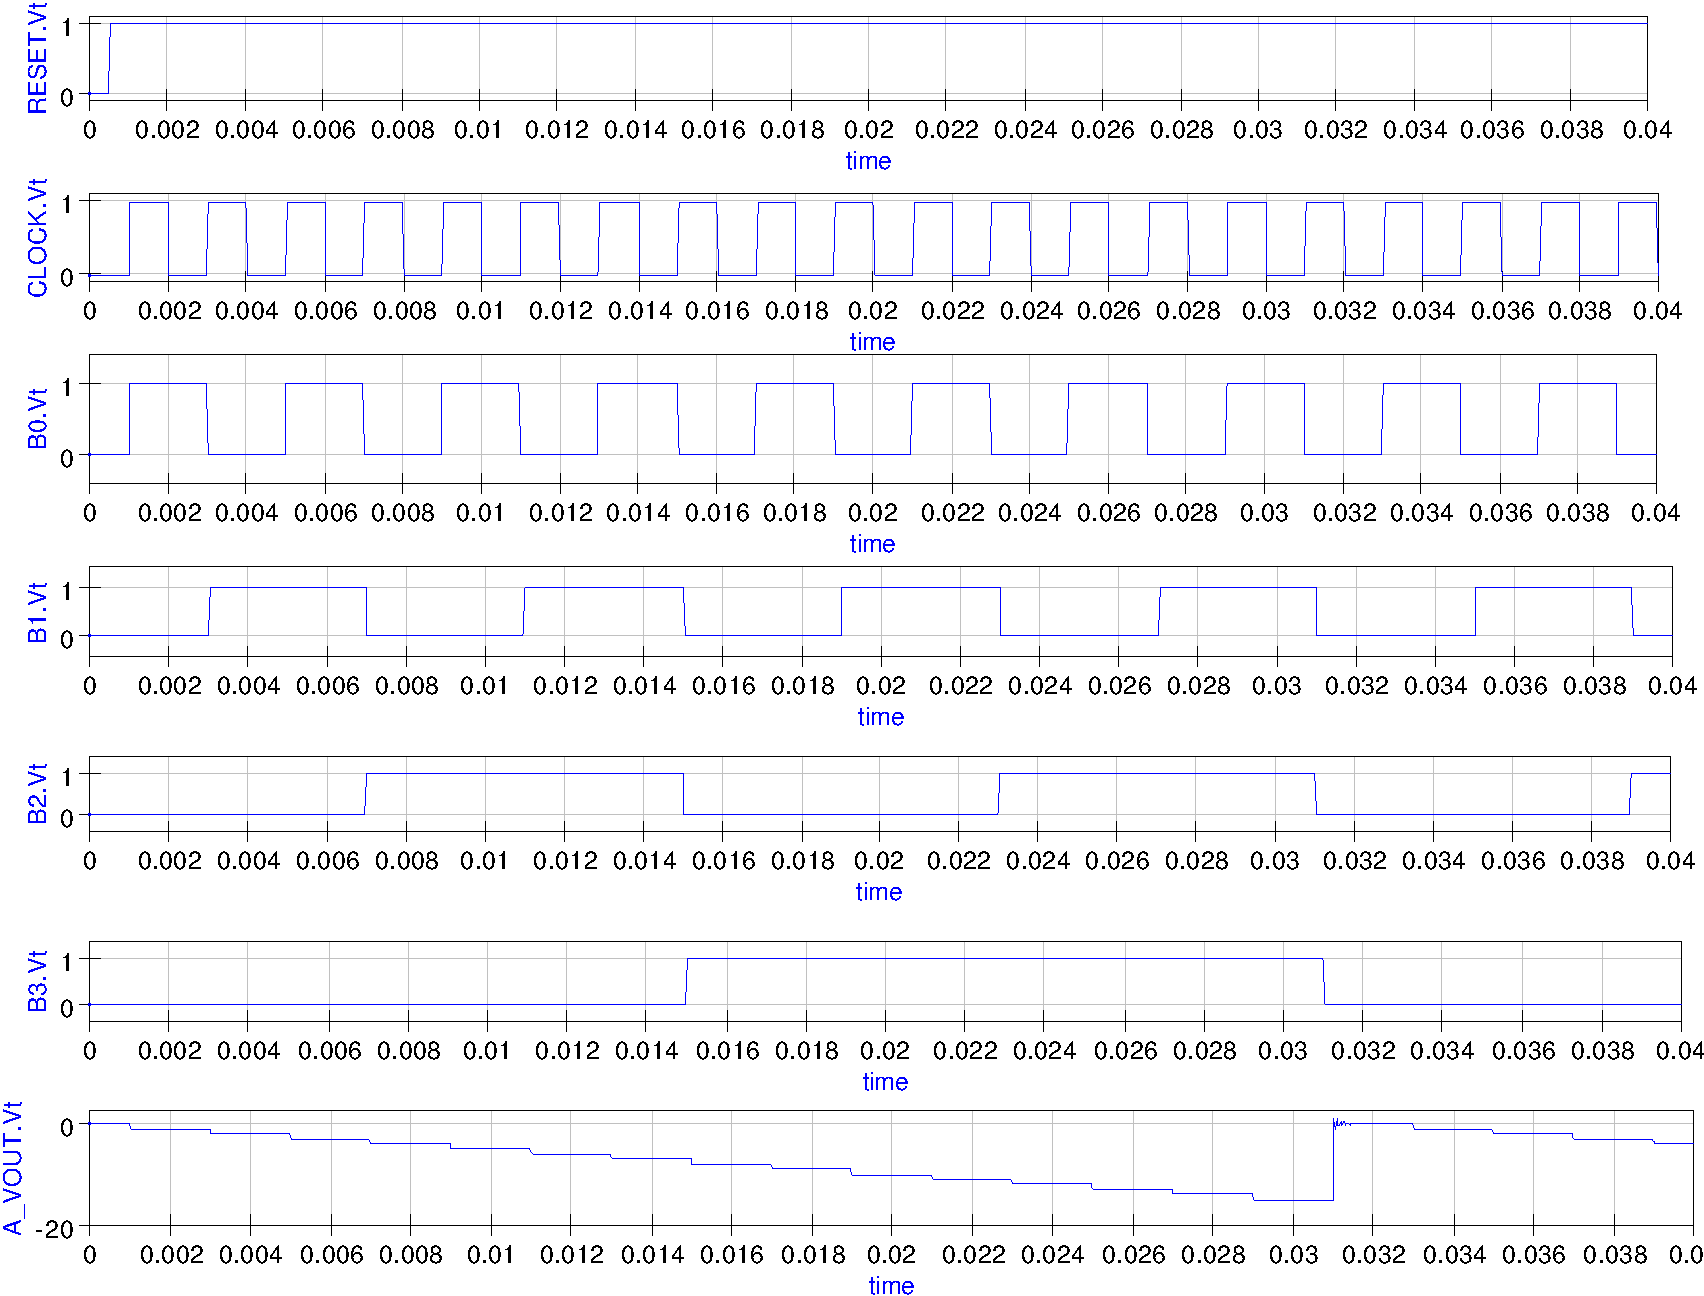
\includegraphics[width=1.0\linewidth]{fig24}
% fig18.pdf: 72dpi, width=28.86cm, height=21.55cm, bb=0 0 818 611
        \caption{Digital TimeList waveforms for the circuit shown in Fig.~\ref{fig:fig23}}
        \label{fig:fig24}
\end{figure}
\begin{figure}[ht]
  \centering
	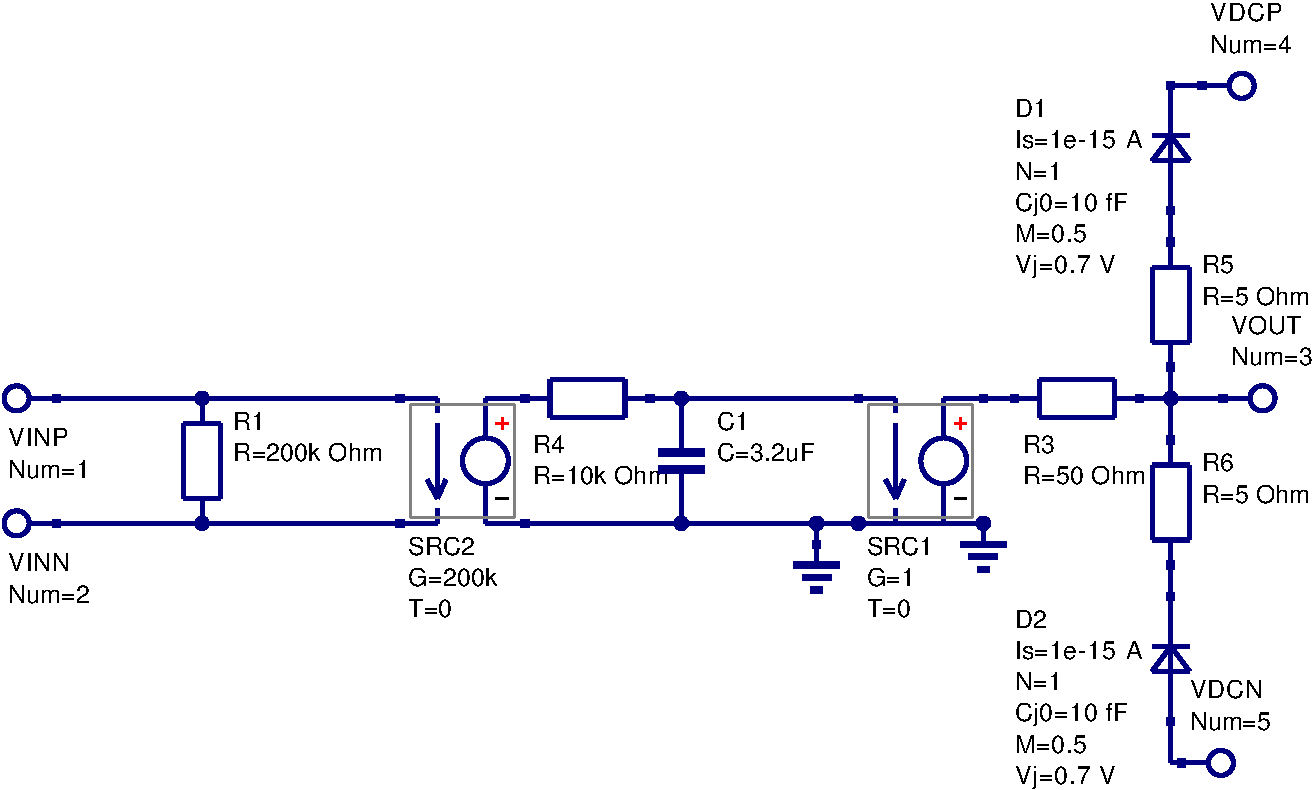
\includegraphics[width=0.9\linewidth]{fig25}
% fig18.pdf: 72dpi, width=28.86cm, height=21.55cm, bb=0 0 818 611
\caption{Operational amplifier model with Rin = 200k $\Omega$, pole frequency = 5Hz, DC differential gain = 200k and Rout = 50 $\Omega$}
        \label{fig:fig25}
\end{figure}
\end{itemize}

\tutsection{End Note}

The examples described in these notes were all simulated using the
latest CVS code version of Qucs. Since release of version 0.0.8, Qucs
has matured enough to allow it to be used for mixed-mode simulation
and many of the known bugs in Qucs 0.0.8 will be corrected with the
release of Qucs 0.0.9 some time in the future.  Release 0.0.9 will
represent another important step in the development of a truly
universal simulator.  However, much more work needs to be done on the
development of models for use across the different physical
domains. My thanks to Michael Margraf and Stefan Jahn for all their
hard work in correcting the bugs which surfaced while the examples
presented in this tutorial note where being tested.





\tutend
